
\documentclass[a4paper]{article}

\usepackage[utf8]{inputenc}	% Flere sprog tegnsæt (fx æøå)
\usepackage[english]{babel}	% Engelsk orddeling og caption tekst
\usepackage[T1]{fontenc}		% Brug 8-bit front
\usepackage{lmodern}		% Vektor front

\usepackage{graphicx}	% Kompatibilitet til visning af pixel billeder (.png, .jpg, .gif)
\usepackage{epstopdf}	% Kompatibilitet til visning af vector billeder (.eps)
\usepackage{float}		% TIllader H som positions parameter
\usepackage{mathtools}	% Det meste matematik (indeholder ams­math og rettelser)
\usepackage{amssymb}	% Flere matematiske symboler
\usepackage{xfrac}		% Flere fracs (\sfrac{}{})
\usepackage{qtree}		% Tableau træ
\usepackage{listings}	% Indsæt code
\usepackage{fancyhdr}	% Side hoved og sidefod
\usepackage{todonotes}	% Cool todo notes, [disable] skjuler todos
\usepackage{parskip}	% Tillader paragraph vertical margin
\usepackage{url}		% Tillader \url formatering
\usepackage{subcaption}	% Tilader subfigure og subtable samt captions i dem
\usepackage{sectsty}
\usepackage{nth}
\usepackage{csquotes}	% Anbefalet package for BibLaTeX
\usepackage[backend=bibtex,style=ieee]{biblatex}				% Benyt BibLaTeX til formatering
\usepackage[bookmarks,bookmarksnumbered,hidelinks]{hyperref} % clickable pdf (til sidst)

%listing settings, æøå support, font config, line number, left lines
\lstset{
    breakatwhitespace=false, breaklines=true,
    inputencoding=utf8, extendedchars=true,
    literate={å}{{\aa}}1 {æ}{{\ae}}1 {ø}{{\o}}1 {Å}{{\AA}}1 {Æ}{{\AE}}1 {Ø}{{\O}}1,
    keepspaces=true, basicstyle=\small\ttfamily,
    frame=L, numbers=left, numberstyle=\scriptsize\color{gray},
} 

% Referencer bliver i to trin, #section.#count
\numberwithin{equation}{section}
\numberwithin{figure}{section}
\numberwithin{table}{section}

\addbibresource{sources.bib}					% Tilføjer sources.bib som reference katalog
\setcounter{secnumdepth}{5}					% Tæl paragraph sektioner
\subsubsectionfont{\fontsize{11}{8}\selectfont}		% Gør subsubsection lidt større end paragraph
\setlength{\marginparwidth}{80pt} 				% Mere brede på margin notes og todos
\setlength{\parindent}{15pt}					% Giver lidt luft imellem afsnitene
\setlength{\parindent}{0cm}   					% Deaktiver afsnit indrykning
\DeclareGraphicsExtensions{.pdf,.eps,.png,.jpg,.gif}	% ændre til .png, .jpg for hurtig visning
\DeclareMathOperator*{\argmin}{arg\,min}
\pagestyle{fancy}

\begin{document}

\title{Analysis of Gravity Recovery and Climate Experiment (GRACE) data}
\author{Andreas Madsen – s123598\\Frederik Wolgast Rørbech - s123956}
\date{Deadline: 09:00- 24th of June 2014}
\maketitle

\setcounter{tocdepth}{2}
\pagebreak
\tableofcontents
\pagebreak

%!TEX root=report.tex
\section{Introduction}
Lately, the climate has become a very hot topic. 
In recent times most natural science researchers have reached a consensus;
the globe is heating up and the primary catalyst of this process is human carbon dioxide emission.
One of the consequences of a warmer Earth is melting ice at various locations.
This leads to rising oceans which could cause a lot of damage to lowlands.
In Denmark an example of the latter would be the marsh area in West Jutland.
Thus, an important question is exactly how the process of ice melting is evolving.

Our data source is Gravity and Climate Experiment (GRACE) \cite{GRACE-data-source}. 
GRACE is a government funded research project which began collecting data in 2002, its mission is to track the gravitational changes on Earth.
The data is captured using two satellites trailing each other while orbiting the Earth.
By measuring the distance between the satellites one can estimate the strength of the gravitational field.
Since gravity is caused by mass, the data can be interpreted as reductions or increases in mass, which may be caused by ice melting.

This report will seek to uncover locations, which are experiencing a significant mass gain/loss, using mathematical models. 
In addition to analysis of the spatial variance, variation in the time domain will also be analyzed.
Finally, results and their uncertainties will be commented on.

\section{Problem definition}
Specifically this report will focus on analyzing local mass losses on the surface of the Earth, partially those changes near Greenland and the South Pole.

\begin{itemize}
\item Is the changes accelerating or decelerating?
\item Does it fluctuate?
\item Does ice at the coasts of the South Pole melt as fast as ice at the coasts of Greenland?
\end{itemize}

\todo[inline]{Check that this is answered}


%!TEX root=report.tex
\section{Data}

The GRACE dataset can be downloaded from GRGS \cite{GRACE-data-source}.
This report is based on the Equivalent Water Height (denoted EWH) dataset from release 2 in the GRGS format with a 10-day interval.

This dataset contains quite a few text files, each containing information in both its filename and its content.
The filenames have the format:

\begin{lstlisting}
grid.water.10day_model_minus_RL02MF.19202_19211.txt
grid.water.10day_model_minus_RL02MF.19212_19221.txt
...
\end{lstlisting}

In the filename, the last two numbers (e.g. \texttt{19202\_19211}) are important.
These numbers contain the start and end date for the file content.
Both numbers are the number of days since ``1950-01-01'', where the first number denotes the start date and the last number the end date of the period for the measurements. \cite{GRACE-data-format-dates}

The actual content of each text file should be read as a ``Space Separated Values'' format.
When this is done one will have a $6480 \times 10$ matrix. 
This matrix can then be \texttt{reshape}'ed row-wise into a $180 \times 360$ matrix.
The result is a matrix with decreasing latitude on the rows and increasing longitude on the columns. \cite{GRACE-data-format-grids}

\subsection{Data example}

\begin{figure}[H]
	\centering
	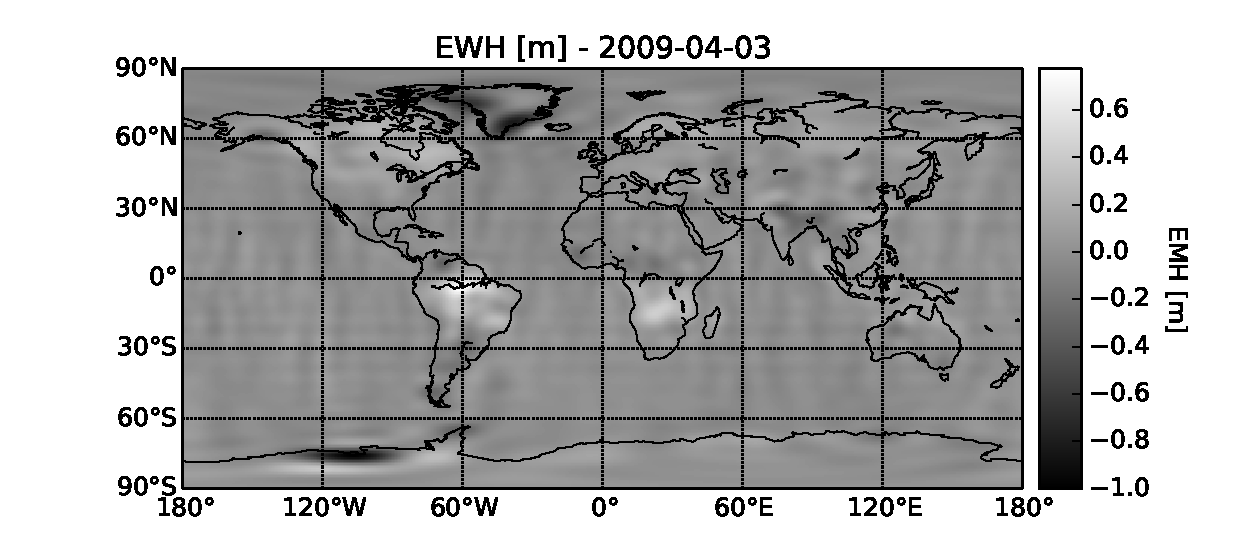
\includegraphics[width=\textwidth]{figures/data-example-world}
	\caption{Plot of the data from 3 April 2009}
	\label{fig:data-example-world}
\end{figure}

\begin{figure}[H]
	\centering
	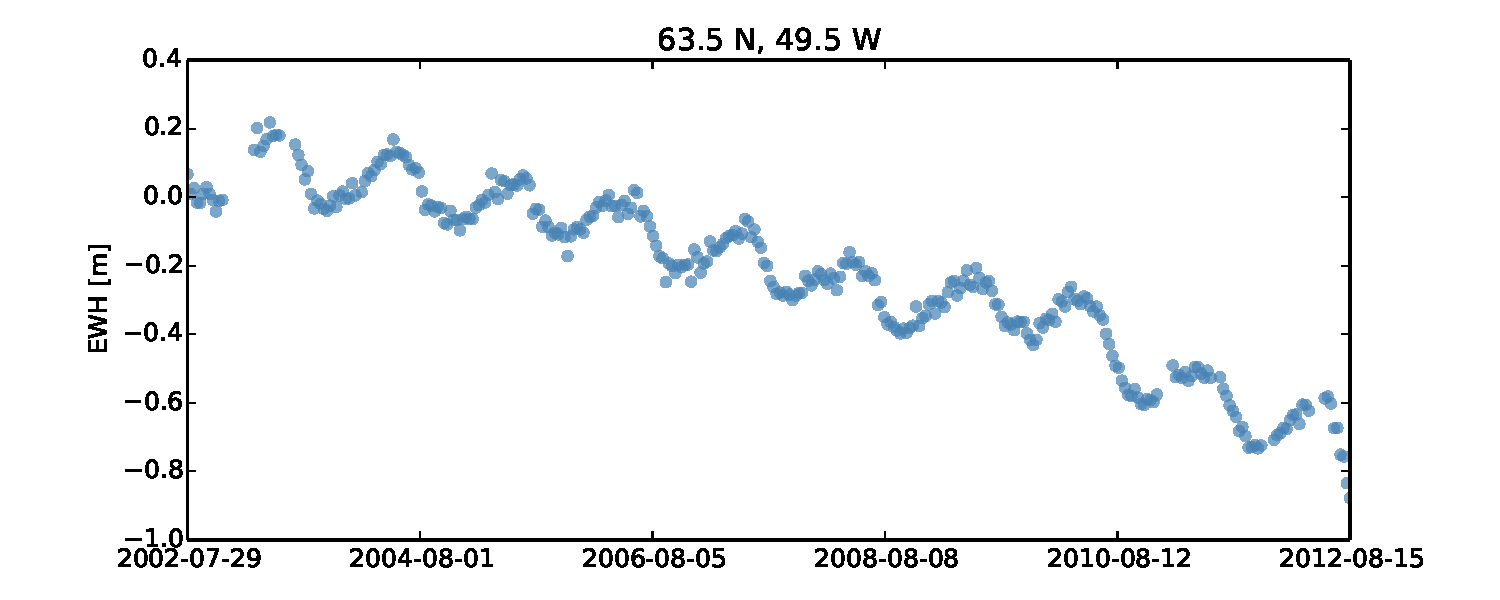
\includegraphics[width=\textwidth]{figures/data-example-scatter}
	\caption{Plot of EWH at 63.5 N 49.5 W, west coast of Greenland.}
	\label{fig:data-example-scatter}
\end{figure}

From Figure \ref{fig:data-example-world} local mass losses at Greenland and the South Pole are seen, this is caused by the ice melting.
A mass increment in South America can also been seen, this is caused by the rain season.
On Figure \ref{fig:data-example-scatter}, mass loss with a yearly periodic trend is seen.


\pagebreak
\section{Theory}
%!TEX root=report.tex
\subsection{SVD}
Singular Value Decomposition (SVD) is a useful method for factorizing matrices.
 According to the SVD-theorem a matrix $X$  can be expressed as
\begin{equation}
X=U \Sigma V^{T}.
\label{eq:theory-svd}
\end{equation}

If the matrix $X$ has the size $m \times n$, the factorized components have the following properties \cite{introduction-to-data-mining}:
\begin{itemize}
\item The columns in $U$ are the eigenvectors of $X X^T$, with the size $m \times m$.
\item The columns in $V$ are the eigenvectors of $X^T X$, with the size $n \times n$.
\item $\Sigma$ is a diagonal matrix, consisting of the square root of the corresponding eigenvalues to the eigenvectors in $U$ and $V$.
It has the size $m \times n$. The square root eigenvalues are also called ``singular values''.
\end{itemize}

In the case where $X$ has many more rows than columns, the $U$ matrix will contain more eigenvectors than are strictly needed to reconstruct $X$ and the $\Sigma$ matrix will have lots of zero-rows.
A so called \textit{economy-size} SVD is therefore often used.
The difference being that all the redundant eigenvectors in $U$ are removed, so it has the size $m \times n$ and the zero-rows from $\Sigma$ are also removed, so its size becomes $n \times n$.

An important property of SVD is that the $V$ matrix contains all eigenvectors and is therefore an orthogonal matrix, for which it is known that
\begin{align}
Q^T = Q^{-1} && Q Q^T = I && Q^T Q = I && \text{, where Q is an orthogonal matrix.}
\end{align}

In the normal SVD (not \textit{economy-size}) $U$ is also a complete orthogonal matrix.
However in \textit{economy-size} some of the columns have been removed, so it is only known that $U^T U = I$.

It is standard procedure to rearrange the matrices in $U \Sigma V^T$, so the largest values in $\Sigma$ appears first in the diagonal.
The reason being that $V$ is a change of basis matrix -- it transforms elements in the original space to a new orthogonal space.
Here the first axis has the largest variance, the second axis has the second highest variance and so on.
The variance described by each axis, is given by the diagonal elements in $\Sigma^2$.
Typically one calculates a percentage called ``variance explained by principal components'' using
\begin{equation}
\rho_{jj} = \frac{\Sigma^2_{jj}}{\sum_{i=1}^n \Sigma^2_{ii}}.
\end{equation}

It is often seen that most of the variance in $X$ can be described using very few eigenvectors, thus one can reduce the dimensionality of a dataset to the most ``principal'' components.
The above mentioned analysis goes under the umbrella term ``Principal Component Analysis (PCA)'', where a ``principal component'' (loadings) should be understood as the axes in the transformed space (i.e., the eigenvectors).

%!TEX root=report.tex
\subsection{OLS}
OLS (Ordinary Least Squares) regression is used for finding the best linear transformation of one or more exogenous variables $X$ so as to predict the dependent variable $Y$. \todo{Improve formulation}
This is done by a matrix-vector product between a $\beta$ vector and $X$.
Since $X$ can be custom tailored for various purposes it is often referred to as the design matrix.
\begin{align}
Y=X \beta +\epsilon && \text{, where } \mathrm{E}[\epsilon] = 0 \text{ and } \mathrm{D}[\epsilon] = \mathrm{D}[Y] = \sigma^2 I .
\end{align}

In the equation above the $\beta$-vector is the unknown parameter which needs to be determined while  $\epsilon$ is a vector containing the residuals which the model cannot account for.
Often the purpose of OLS is to predict $Y$, but in this case we want to analyze the individual $\beta_i$ elements.

\subsubsection{The solution to the OLS problem}
As the name sugest, the OLS method minimizes the sum of squared residuals ($\epsilon^T \epsilon$).
It is seen directly that $\epsilon = Y - X \beta$ and thus the following is obtained
\begin{equation}
\begin{split}
\epsilon^T\epsilon&=(Y-X\beta)^T (Y-X\beta)\\
&=(Y^T-\beta^T X^T) (Y-X\beta) \\
&=Y^T Y-\beta^T X^T Y-Y^T X \beta + \beta^T X^T X \beta \\
&=Y^T Y- 2\beta^T X^T Y+ \beta^T X^T X \beta.
\end{split}
\end{equation}

One can now differentiate with respect to the $\beta$ vector
\begin{equation}
\begin{split}
\frac{\partial \epsilon^T\epsilon}{\partial \beta}&=-2 X^T Y+2X^T X \beta=2(-X^T Y+X^T X \beta).
\end{split}
\end{equation}

Now  $\epsilon^T \epsilon$'s minimum is given by solving for $\frac{\partial \epsilon^T\epsilon}{\partial \beta} = 0$
\begin{equation}
\begin{split}
\frac{\partial \epsilon^T\epsilon}{\partial \beta} = 0 \Rightarrow 2(-X^T Y+X^T X \hat{\beta}) &= 0 \\
X^T X \hat{\beta}&=X^T Y \\
\hat{\beta}&=(X^T X)^{-1} X^T Y.
\end{split}
\end{equation}

The solution above is formally correct \cite[p.~12]{statistical-learning}, but if $X$ is badly conditioned $(X^T X)^{-1}$ might not be numerically stable (i.e. if the columns in $X$ are highly correlated leading to a near singular $X^T X$) \cite[p.~8]{aasbjerg-ls}.
To avoid this problem $X$ should be factorised and the solution reformulated; in this report we will exclusively do this using SVD
\begin{equation}
\begin{split}
\left( U \Sigma V^T\right)^T \left(U \Sigma V^T\right) \hat{\beta} &= \left(U \Sigma V^T\right)^T Y \\
\left( V \Sigma^2 V^T \right) \hat{\beta} &= V \Sigma U^T Y \\
\hat{\beta} &= \left( V \Sigma^2 V^T \right)^{-1} V \Sigma U^T Y \\
\hat{\beta} &= V \Sigma^{-1} U^T Y.
\end{split}
\end{equation}

It should be noted, that when multiple $\hat{\beta}$ vectors need to be calculated (one vector for each spatial location on the surface) optimization is possible, by arranging $Y$ as a matrix with each column corresponding to a location.
$\hat{\beta}$ will then be a matrix containing all solutions instead of a vector containing only one solution.

\subsubsection{The ``Hat" matrix}
In the special case of the GRACE data, the $X$ matrix is identical for every position. This can be exploited by constructing a hat matrix $H$ which only depends on $X$ and projects $Y$ onto $\hat{Y}$ (puts the hat on $Y$).
\begin{equation}
\begin{split}
\hat{Y} &= X \hat{\beta} \Rightarrow \hat{Y} = X V \Sigma^{-1} U^T Y \\
\hat{Y} &= H X \quad \text{, where } H = X V \Sigma^{-1} U^T.
\end{split}
\end{equation}

As earlier with $\beta$, the hat matrix can be calculated for all $Y$ vectors by horizontally stacking $Y$ to form a matrix.

An important property of the $H$ matrix is that it is idempotent ($H^2 = H$).
This is because $H$ is a projection matrix which projects $Y$ onto $\hat{Y}$.
Projecting $Y$ onto $\hat{Y}$ and then projecting again onto $\hat{Y}$, will obviously not change anything, because one is already in the $\hat{Y}$-plane.

\subsubsection{Root Mean Squared Error}

``Root Mean Squared Residuals'' (RMSE) is an indicator of how good an $Y$ estimate is.
It can be calculated as
\begin{equation}
\hat{\sigma} = \sqrt{\frac{\left(Y - \hat{Y}\right)^T \left(Y - \hat{Y}\right)}{N-p}},
\end{equation}

where $p$ is the number of parameters (elements in $\beta$) and $N$ is the number of observations (elements in $Y$).
RMSE is an estimate for the standard deviation of $Y$ \cite[theorem~3.4]{time-series-analysis} thus the symbol $\hat{\sigma}$.


\subsubsection{The variance of $\hat{Y}$}

The dispersion (variance-covariance) of $\hat{Y}$ can be calculated as
\begin{equation}
\mathrm{D}[\hat{Y}] = \mathrm{D}[H Y] = H \mathrm{D}[Y] H^T = \sigma^2 H^2 = \sigma^2 H.
\end{equation}

The variance of $\hat{Y_i}$ is given by the diagonal elements in $\mathrm{D}[\hat{Y}]$
\begin{equation}
\mathrm{Var}[\hat{Y_i}] = \sigma^2 H_{ii}.
\end{equation}

Because $\sigma^2$ is a scalar, the diagonal in $H$ is important to examine, since it can reveal potential elements (in our case points of time) with high variance in the predictions.

\subsubsection{The dispersion of $\hat{\beta}$}

The dispersion of $\hat{\beta}$ is calculated as \cite[theorem~3.2]{time-series-analysis}:
\begin{equation}
\mathrm{D}[\hat{\beta}] = \sigma^2 (X^T X)^{-1} = \sigma^2 V \Sigma^{-2} V^T
\end{equation}

Seeing as $\sigma^2$ is a scalar and dependent of $Y$, a similar spatial independent expression can be made, by removing the scalar $\sigma^2$  factor, thus looking exclusively at $V \Sigma^{-2} V^T$.

\subsubsection{p-values for $\hat{\beta}$}

To calculate p-values for OLS parameters the student's t-distribution is used, with the t-score \cite[p.~172]{time-series-analysis}
\begin{align}
\mathrm{t} = \frac{\hat{\beta_i}}{\mathrm{SD}[\hat{\beta_i}]} && \text{where: } \mathrm{SD}[\hat{\beta_i}] = \sqrt{\mathrm{Cov}[\hat{\beta}]_{ii}} = \hat{\sigma} \sqrt{ (V \Sigma^{-2} V^T)_{ii} }.
\end{align}

Now by plugging the t-score into the Student's Cumulative T-Distribution Function ($\Phi_t$) with $N - p$ degrees of freedom, we get
\begin{equation}
p = 2 \cdot \Phi_t\left(\mathrm{abs}(t), N-p\right)
\end{equation}

The null-hypothesis is that $\beta_i = 0$ and th  e alternate hypothesis is $\beta_i \not = 0$.

%!TEX root=report.tex
\subsection{The design matrix}
In OLS regression, a linear combination of the columns in the design matrix $X$, is used to predict $Y$.
As a starting point, the only values in $X$ are a column of ones (to fit an intercept) and a column containing the observed time $t$

\begin{equation}
X = \left[\begin{matrix} \mathbf{1} & \mathbf{t} \end{matrix}\right].
\end{equation}
In the above case one would predict $\hat{Y}$ as $\beta_1 + \beta_2 t$ where $\beta_1$ will correspond to the intercept (uninteresting) and $\beta_2$ will correspond to the speed of mass gain.
From this it follows naturally to include the acceleration by adding a column

\begin{equation}
X = \left[\begin{matrix} \mathbf{1} & \mathbf{t} & \frac{1}{2} \mathbf{t}^2 \end{matrix}\right]
\end{equation} 
From Fourier analysis it is known that functions can be approximated by infinite sums of the trigonometric functions sines and cosines.
Trigonometric functions are periodic in their behavior and thus are able to model periodic signals in the function that one wishes to approximate.

In the GRACE dataset, however, the measurements are recorded with a frequency of $\frac{1}{10}$ days.
The Nyquist-Shannon sampling theorem states that one cannot find periodic signals below the Nyquist frequency which is given as half of the sample frequency. 
Therefore an infinite sum is not suited for approximating the function. 
Instead it will be assumed that the maximal frequency in the data has a period of a year ($365.242$ days) while the minimal frequency will have 18 periods per year since  $\sfrac{365.242}{18} \approx 20.29$. Hence it follows that the final design matrix will be given as
\begin{equation*}
\resizebox{\textwidth}{!}{$
X = \left[\begin{matrix}
	\mathbf{1} &
	\mathbf{t} &
	\frac{1}{2} \mathbf{t}^2 &
	\cos\left( \dfrac{2 \pi}{\frac{365.242}{1}} \mathbf{t} \right) &
	\sin\left( \dfrac{2 \pi}{\frac{365.242}{1}} \mathbf{t} \right) &
	\cdots &
	\cos\left( \dfrac{2 \pi}{\frac{365.242}{18}} \mathbf{t} \right) &
	\sin\left( \dfrac{2 \pi}{\frac{365.242}{18}} \mathbf{t} \right)
\end{matrix}\right].
$}
\end{equation*}

From this it's seen that the angular frequency is $\omega_i =  \dfrac{2 \pi}{\frac{365.242}{i}}$

%!TEX root=report.tex
\subsection{Phase and Amplitude}

The $\mathbf{\beta}$ parameters in the OLS problem are linear combinations of $\cos(\omega_i t)$ and $\sin(\omega_i t)$ function pairs.
However from a physics perspective having both $\cos(\omega_i t)$ and $\sin(\omega_i t)$ for the same $\omega_i$ have no meaning.
Instead one should convert the $\beta$ parameters for the trigonomic functions intro amplitude and phase for a single periodic function $A_i \cos(\omega_i t + \phi_i)$.
This is done by using Ptolemy's theorem
\begin{equation}
A_i \cos(\omega_i t + \phi_i) = A_i \cos(\phi_i) \cos(\omega_i t) - A_i \sin(\phi_i) \sin(\omega_i t).
\end{equation}

Comparing with the linear combination from OLS
\begin{align}
\hat{Y} = \cdots + \beta_{c,i} \cos(\omega) + \beta_{s,i} \sin(\omega) + \cdots
\end{align}
it's see that
\begin{align}
\beta_{c,i} = A \cos(\phi_i) && \text{ and } && \beta_{s,i} = A \sin(\phi_i).
\end{align}

By dividing these two equations with each other, $\phi_i$ can be calculated as \todo{This is not the one used in the code. (Sign diffrence)} 
\begin{equation}
\frac{- A_i \sin(\phi_i)}{A_i \cos(\phi_i)} = \frac{\beta_{s,i}}{\beta_{c,i}} \Rightarrow \phi_i = \arctan\left(-\frac{\beta_{s,i}}{\beta_{c,i}}\right).
\end{equation}

To isolate $A_i$, square both equations and add them together:
\begin{equation}
A_i^2 \cos(\phi_i)^2 + A_i^2 \sin(\phi_i)^2 = \beta_{c,i}^2 + \beta_{s,i}^2 \Rightarrow A_i = \sqrt{\beta_{c,i}^2 + \beta_{s,i}^2}.
\end{equation}

The result can be plotted with a circular color scale for the $\phi_i$ and $A$ is then the intensity of the color.

%!TEX root=report.tex

\subsection{OLS with autocorrelated residuals}

In OLS it is assumed that the residuals between different observations are uncorrelated. However since our data is a time series this assumption does most likely not hold. This can also be confirmed with the Durbin-Watson test statistic \cite[p.~173]{autocorrelation-kousgaard}. This test statistic is calculated using
\begin{equation}
d = \frac{\sum_{i=2}^n \left( \hat{\epsilon}_i - \hat{\epsilon}_{i-1} \right)^2}{ \sum_{i=1}^n\hat{\epsilon}_i^2 }
\end{equation}

which lies between 0 and 4. If $d$ is close to 0 the residuals $\hat{\epsilon}_i$ and $\hat{\epsilon}_{i-1}$ are correlated positively, if close to 4 the residuals are negatively correlated. The purpose of this method is to reduce the correlation between the residuals, the Durbin-Watson test statistic should then become 2.

When the residuals are correlated, one gets bad estimation of the variance of the residuals $\hat{\sigma}_\epsilon^2$. This in turn leads to bad interference statistics, such as misleading p-values.

To correct for the correlated residuals, one can use a general least squares (GLS) regression. This uses a $\Sigma$ matrix there will correct for the correlated residuals
\begin{equation}
\min_{\beta, \rho}\ (Y-X\beta)^T \Sigma^{-1}(Y-X\beta),
\label{eq:theory-olsar-min}
\end{equation}

where $ \Sigma^{-1}$ is given as
\begin{equation}
\Sigma^{-1}  = \begin{bmatrix}
1         & -\rho         & 0               & \cdots & 0              & 0         \\
-\rho   & 1+\rho^2 & -\rho         & \cdots & 0               & 0         \\
0         & -\rho         & 1+\rho^2 & \cdots &0                & 0         \\
\vdots & \vdots      & \vdots       & \ddots & \vdots      & \vdots \\
0         & 0               &0                & \cdots & 1+\rho^2 & -\rho    \\
0         & 0               &0                & \cdots &-\rho          & 1
\end{bmatrix}
\end{equation}

The optimization problem \eqref{eq:theory-olsar-min} is nonlinear and there is no closed form solution to this problem. However when keeping $\rho$ constant the $\beta$ parameters can be estimated using  General Least Squared, which is similar to OLS but with a constant $\Sigma$ matrix and have the solution \cite[p.~38]{time-series-analysis}
\begin{equation}
\hat{\beta} = (X^T \Sigma^{-1} X)^{-1} X^T \Sigma^{-1} Y.
\end{equation}

This should then be rewritten using SVD, to account for a near singular $X^T \Sigma^{-1} X$ matrix.

Similarly when $\beta$ is kept constant, $\rho$ can be estimated with  \cite[p.~178]{autocorrelation-kousgaard}
\begin{equation}
\hat{\rho} = \frac{ \sum_{i=2}^n \hat{\epsilon_i}\hat{\epsilon}_{i-1} }{ \sum_{i=2}^{n-1} \hat{\epsilon_i}^2 }.
\label{eq:theory-olsar-rho}
\end{equation}

A practical way of solving the problem with respect to both $\beta$ and $\rho$, looks as follows:
\begin{enumerate}
\item initialize by letting $\rho=0$
\item Iterate: \begin{enumerate}
	\item Keep $\hat{\rho}$ constant and estimate $\beta$ using as a WLS problem.
	
	\item Keep $\hat{\beta}$ constant and estimate $\rho$ using \eqref{eq:theory-olsar-rho}.
	
	\item Repeat until convergence of $\rho$ or until some predetermined upper iteration boundary is met.
\end{enumerate}
\end{enumerate}

%!TEX root=report.tex
\subsection{Least angular regression (LAR)}
The LAR model is almost equivalent to the linear regression, except that instead of only minimizing the sum of squares, an $\ell^1$ norm penalty as added on the $\hat{\beta}$-vectors coefficients.
\begin{align}
\min_{\hat{\beta}}\ (Y - \hat{Y})^T (Y - \hat{Y}) \quad \text{subject to} \quad ||\hat{\beta}||_1 \le s
\end{align}

The LAR algorithm \cite{LAR-algorithm} solves this problem by initially letting all the $\beta$ coefficients be zero.
It then finds the attribute, $b_1$, with the highest absolute correlation with the dependent variable Y and increases $b_1$  (or decreases depending on the sign of the correlation)
until it reaches a point where another attribute $b_2$ has as much  correlation with the residuals $R=Y-\hat{Y}$ as  $b_1$ has.
At this point the algorithm then increases/decreases both $b_1$ and $b_2$ in their joint direction until another attribute $b_i$ has the highest residual correlation.
This process can then be continued until there is no benefit in increasing any of the $b_i$s - that is, the full LAR solution is equivalent to the linear regression.
It should also be noted that if a coefficient crosses 0 in a iteration (step),
that coefficient should be set to 0, and the regression direction \todo{Allan marks this} should subsequently be recomputed.

So why might one use LAR instead of for example the LASSO model? 
When using the LASSO one has to chose a specific value of $s$ to get one solution.
However, in the LAR model you actually get the full solution path which means that you can find all the LASSO solutions instead of having to do multiple LASSO with different regularization parameters ($s$).

%!TEX root=report.tex
\subsection{Basis expansion}

Basis expansion is done by adding more columns to design matrix. Let us first motivate why this might be needed.

\subsection{Motivation}
It has previously been described how the design matrix $X$ was constructed such that we had 
\begin{equation*}
\resizebox{\textwidth}{!}{$
X = \left[\begin{matrix}
	\mathbf{1} &
	\mathbf{t} &
	\frac{1}{2} \mathbf{t}^2 &
	\cos\left( \dfrac{2 \pi}{\frac{365.242}{1}} \mathbf{t} \right) &
	\sin\left( \dfrac{2 \pi}{\frac{365.242}{1}} \mathbf{t} \right) &
	\cdots &
	\cos\left( \dfrac{2 \pi}{\frac{365.242}{18}} \mathbf{t} \right) &
	\sin\left( \dfrac{2 \pi}{\frac{365.242}{18}} \mathbf{t} \right)
\end{matrix}\right].
$}
\end{equation*}
The problem with the above $X$ is that the periodic columns assumes the pattern accounts for the entire period. This causes problems in areas such as Denmark, where the winter comes later than ``usual'', or the summer is much colder/warmer etc..

This leads to higher variance of the residuals which decreases the accuracy of the velocity and acceleration parameter of the model. By adding columns to the design matrix, such that the periodic pattern is only assumed extend over one period, the accuracy can be improved.

\subsection{The Hinge-function}

One can achieve this basis expansion is by virtue of the hinge-function
\begin{equation}
f(x - \zeta)_+ = \begin{cases}
  f(x - \zeta) & \text{if } x - \zeta \ge 0 \\
  0                 & \text{otherwise}
\end{cases} \quad \forall x \in \mathbb{R}, \zeta \in \mathbb{R}
\end{equation}
$\zeta$ denotes the ``knot'' between the zero part and the $f$ part. By choosing $f$ and adding the hinge function to the design matrix, a basis expansion where terms are only active for some parts of the time series is obtained.

When $f$ is a polynomial one achieve a piecewise polynomial which is called a spline.
In this case each hinge function is guaranteed to be continuous and it can be shown that the spline's derivatives are continuous to order $M-2$ where $M$ is the degree of polynomial $f$ \cite[p.~144]{statistical-learning}. When dealing with polynomials, splines which are continuous up to and including its second order derivatives are called \textit{cubic splines} and they generate nicely looking curves when performing the regression. \cite[p.~143]{statistical-learning}.

\subsubsection{Knots and trigonometric functions}
To model each year with different behavior, in essence all that is needed is to create 9 knots (10 intervals requires 9 splits) and construct the hinge functions.
However, since the functions being used are sines and cosines, there is no guarantee of continuity at the knots (only continuity if the trigonometric function evaluates to zero at the knot).
In grim cases, when multiple discontinuous functions are combined, one can end up with cusps, that is a steep descent/ascend followed by the opposite movement in rapid succession.
If this phenomenon becomes too large, one should consider rejecting the model, this will be discussed in the result section. 

%!TEX root=report.tex
\subsection{Time Series Analysis}

In time series analysis one attempt to find a model for predicting data. This is different form the OLS analysis there tries to estimate the trends in the data, such as velocity and acceleration. Once such model is found, it should be validated by analyzing the residuals. These residuals must be approximately white noise \cite[p.~130]{time-series-analysis}, otherwise the model is invalid. 

\subsubsection{ARIMA}

ARIMA is the name of the stochastic model used. The detail will not be discussed here, instead we refer to \cite[p.~130]{time-series-analysis}.

In short ARIMA uses the previous values with some weight to predict. Which values are used is denoted by the following notation:
\begin{equation}
(p, d, q) \times (P, D, Q)_s
\end{equation}

$p$ is the highest lags of actual measurements used and $q$ is the maximum amount of lags in residuals used. The $d$ part indicates how many difference operators there should be used to transform the data. $(P, D, Q)$ is completely similar, but steps not by one lag but by $s$ lags. This allows for seasons trends such as an yearly pattern.

\subsubsection{ACF and PACF}
 
ACF and PACF is a measure of correlation between different time lags and is used to make a qualified guess about how the predicting model should look like. 
For how these are estimation please see \cite[p.~146]{time-series-analysis}.

When ACF and PACF have been estimated, rules \cite[table~6.1]{time-series-analysis} for how the stochastic model should look can be applied.
Typically when dealing with complex models, this becomes and iterative process.
Where one will calculate the ACF and PACF on the suggested model and then adjust the model accordingly.

\subsection{Ljung-Box test}

The null hypothesis for the Ljung-Box is ``The data is independently distributed''. Thus a low p-value means that the residuals aren't white noise.

The Ljung-Box is a $\chi^2$ test with the statistical value:
\begin{equation}
Q = n \cdot (n + 2) \sum_{k=1}^h \frac{\hat{\rho}_k^2}{n - k}
\end{equation}

$n$ is the number of observations. The parameter $h$ is the highest lag in the ACF there should be considered. The $\chi^2$ statistics, have $h - (p + q + P + Q)$ degrees of freedom.

%!TEX root=report.tex
\subsection{K-means clustering}

Clustering is the process of grouping or dividing a set of objects into disjunct subsets, such that objects in each cluster are similar.
All clustering methods are unsupervised learning methods, thus there is no ``correct'' answer.
It have been shown that given a set of objects, humans also differ in their choice of clusters.

Since similarity is an imprecise term, one uses a distance function to use as a Dissimilarity Measure $d$.

There are 4 conditions a distance function $d$ must satisfy, they are all derived from the norm definition \cite[p.~30]{math-4}:
\begin{align}
\text{(i) }   & d(p_1,p_2) \ge 0 && \forall \ p_1, p_2 \in V \\
\text{(ii) }  & d(p_1,p_2) \le d(p_1, p_3) + d(p_3, p_2) && \forall \ p_1, p_2, p_3 \in V \\
\text{(iii) } & d(p_1, p_2) = d(p_2, p_1) && \forall \ p_1, p_2 \in V \\
\text{(iv) } & d(p_1, p_2) = 0 \Leftrightarrow p_1 = p_2 && \forall \ p_1, p_2 \in V
\end{align}

Given a distance measure the total cluster variance $C^{*}$ can be calculated as
\begin{equation}
C^{*}=\sum^K_{k=1} N_k \sum_{i \in C_k} D(x_i, \mu_k).
\end{equation}
Here $\mu_k$ denotes the k\textsuperscript{th} cluster center (also called a centroid), $N_k$ the number of observations in cluster $k$ and $C_k$ denotes the subset with all the points in the cluster $k$.

In this analysis the Euclidean distance $D(x_i, x_j) = ||x_i - x_j||_2$ has been chosen as the dissimilarity measure.
K-means is then the chosen algorithm for minimizing $C^{*}$ given $K$ clusters.
The k-means method as the dataset size is $(lat \cdot lon, days) = (64800,341)$ and k-means is fairly quick to converge and calculate.

K-means makes a single big assumption about the clusters being hyper dimensional sphere. But beyond this K-means is a simple iterative algorithm:
\begin{enumerate}
	\item Initialize cluster centroids
	\item Iterate until centroid convergence:
	\begin{enumerate}
		\item Given the current set of centroids, reassign each observation to the closest centroid using the distance function.
		\item Using the current cluster assignment $C_k\ \forall k$, minimize $C^{*}$ by recomputing the centroids for each cluster as the mean of points in each cluster.
	\end{enumerate}
\end{enumerate}

\subsubsection{Gap-statistics}

The big issue with clustering is that there is no obvious way of selecting the amount of clusters $K$. In this analysis the Gap-statistics \cite[p.~519]{statistical-learning} as proposes by Hastie, Tibshirani and Firedman is used.

First calculate the cluster dissimilarity using $K$ clusters \cite{gap-statistic}
\begin{equation}
W_K = \sum_{k=1}^K \frac{1}{2 N_k} \sum_{x_i\in C_k} \sum_{x_j\in C_k} ||p_i - p_j||_2^2 = \sum_{k=1}^K \sum_{x_i\in C_k} ||p_i - \mu_k||_2^2.
\end{equation}

Given the quantity $W_k$ one can then calculate a gap $G$ by simulating $b$ datasets from a random uniform distribution and calculating the gap as
\begin{equation}
G(k) = \mathrm{E}[\log(W_k)] - \log(W_k),
\end{equation}
where the expectation $\mathrm{E}[\log(W_k)]$ can be estimated by the mean over the $b$ simulated datasets. That is the gap statistics tries to avoid overfitting by comparing the cluster gain on a dataset where there are no clusters (uniformly distributed).

The amount of clusters $K$ is then minimized under the condition
\begin{equation}
K^{*} = \argmin_K \left\{ K \ | \ G(K) \ge G(K + 1) - s'_{K+1} \right\}.
\end{equation}

Here $s'_{K+1}$ is the standard error on the $b$ samples calculated as 
\begin{equation}
s'_{K} = \mathrm{SD}[\log(W_k)] \sqrt{1+\frac{1}{b}}.
\end{equation}

%!TEX root=report.tex
\subsection{Gaussian Mixture Model (GMM)}
The GMM is a more advanced clustering model than K-Means. 
The main advantage is that GMM allows for hyper elliptical clusters. This uses gaussian kernels with its the shape described in a covariance matrix. A result similar to K-means could be obtained by forcing this covariance matrix to be the identity matrix.

Restrictions on the covariance matrix (i.e. shared covariance, diagonal covariance, spherical covariance etc.) can easily be applied in GMM and is quite common. In this analysis however, no covariance restrictions will be used.

In the GMM the assumption is that data comes from a single density function.
The density function is assumed to be a combination (mixture) of $K$ Gaussian PDFs where K is finite and denotes the number of mixture components (i.e. clusters).

Each mixture component has a centroid (the mean), a covariance matrix and a mixing weight.
The sum of mixing weights across components has to be one for the GMM to constitute an actual pdf.

To estimate the model parameters several different methods exists. The most common and is the expectation maximization (EM) algorithm which is quite complex and thus wont be described here. To the curious reader we recommend \cite[p.~214,272,463]{statistical-learning}).

In practice if K is large and the vector space $X$ is high dimensional, estimation of the model parameters will take too much computing power, and even if one get model parameters to converge, the degrees of freedom will be low.
In our case the input space would be 341-dimensional (341 observations in time per location) and thus a dimensionality reduction of some kind is needed. 

\subsubsection{Dimensionality reduction}
In many cases when dealing with high dimensional data, most of the data lies on a lower dimensional manifold. 
Different methods exists to try to identify such manifolds, but in this analysis the previously described technique PCA will be used. \todo{Now we use kernel PCA, not just linear PCA}
This is done by selecting only the most important principal components from the PCA, thus forcing the data onto a lower dimensional manifold.
The GRACE data contains quite a bit of noise and one might hope that the noise will be primarily contained in its own principal components. Hopefully those PCs will only account for a small amount of the variance in the data. 
Thus when selecting only the most significance PCs some of the noise will be "lost".
This combined with the more flexible GMM over K-Means, will hopefully lead to better clustering.

%!TEX root=report.tex
\subsection{Kernel Principal Component Analysis (Kernel PCA)}

Before delving into kernel methods, the standard PCA method will briefly be recapped. PCA as introduced in this report was done via SVD ($X=U\Sigma V^T$); the columns of $U$ were the eigenvectors of $XX^T$ and the columns of $Z$ where $Z=U\Sigma$ constituted a basis in the PCA-vectorspace ($Z$); these columns were referred to as the principal components (PCs). 
Looking at the dependencies of $U$ it is apparent that the PCs will end up being linear combinations of basis in original input space $X$. 
In most cases this suffices but what if there are no linear relationships in the $X$ space, standard PCA won't be appropriate.
Below is a concrete example

\begin{figure}[H]
	\center
	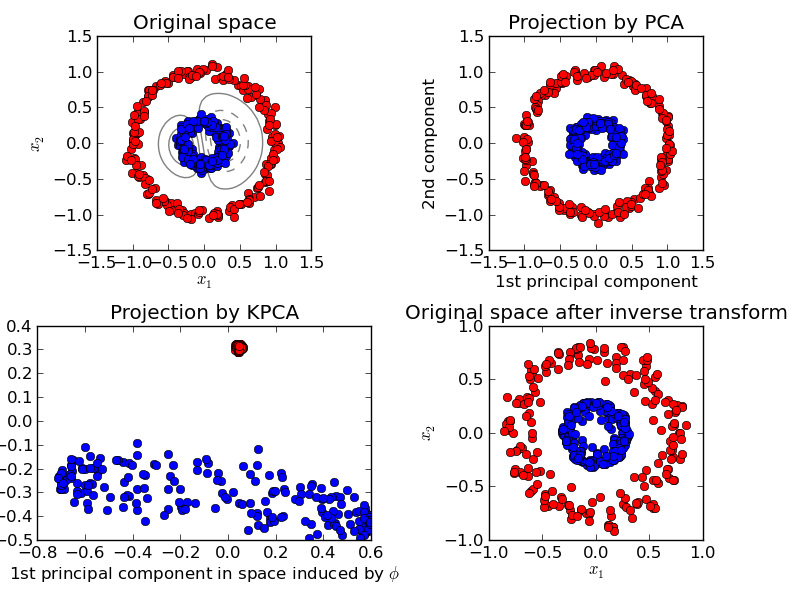
\includegraphics[width=\textwidth]{figures/kernel_pca_example.png}
	\caption{Motivating kernel PCA example. Image courtesy of scikit-learn. http://scikitlearn.org/stable/auto\_examples/decomposition/plot\_kernel\_pca.html }
	\label{fig:motivation_kernelpca}
\end{figure}.
As is seen in the figure above, classes that wasn't linearly separable in the Original space can be become linearly separable in the kernel space. This in turn makes clustering much easier and hopefully improves results.

\subsubsection{The Kernel Trick}

The following two sections are heavily influenced by a video lecture from youtube \cite[from minutes 10-30]{youtube-caltech}. In kernel PCA, instead of working on the inner product $(X,X^T)$ we are interested in using a nonlinear mapping $\Phi: X\rightarrow Y$, such that the singular value decomposition is carried out on $(\Phi(X),\Phi(X^T))=(Y,Y^T)=K(X,X^T)$; this inner product in the $Y$-space is called the kernel. 
So for something to be a valid kernel, all it needs to satisfy is for the kernel to a function of an inner production in some vector space.
For the above to become more clear, let us give an example of a polynomial kernel in a 2-dimensional $X$-space. in the following $X$ is a vector and $X'$ is simply some other vector in the same space as $X$:

\begin{equation}
K(X,X')=(1+X^T X')^2=(1+x_1^T x_1^{'}+x_2^T x_2 ')^2=1+x_1^2 {x_1 '}^2 +2 x_1 x_1 '+2 x_2 x_2 '+2 x_1 x_1 ' x_2 x_2'
\end{equation}

So for the above to actually be a true kernel there would have to be some vector space $Y$ in which the above was an inner product. From the coefficients above it can be deduced that the basis in the $Y$ must be given as
\begin{equation}
(1,x_1^2,x_2^2,\sqrt{2} x_1, \sqrt{2} x_2 , \sqrt{2} x_1 x_2)
\end{equation}
So why is the above important. Imagine if one were to increase the power from 2 to i.e. 100: $K(X,X')=(1+X^T X')^100$. Calculating the kernel in the $X$-space is easy; $(1+X^T X')$ is just a number and raising it to the power of 100 can be done quickly. 
On the other hand if one were to explicitly calculate the kernel as the inner product in the the $Y$-space, you would first have to compute a more than 100-d vector, transpose it, multiply the terms and sum them - i.e. not very efficient and imagine if $X$ had a dimension of 100 instead of 2 - you would end up with too many variables for the computation to be possible.

 All of the above is denoted as the Kernel Trick. It simples is the process of utilizing the fact that the inner product in the $Y$-space can be carried out without knowing the explicit mapping $\Phi$ and as we will show in the next section $\Phi$ can even be a mapping to an infinite dimensional space in which case it would be impossible to actually carry out this transformation.

\subsubsection{The Radial Basis Function (RBF) kernel}
Due to the trigonometric nature of the GRACE data ( remember the fourier expansion with sines and cosines) the appropriate kernel has been deemed to be RBF. The RBF kernel is defined as
\begin{equation}
K(X,X')=exp(-\gamma ||X-X'||^p)
\end{equation}
Now the above can easily be calculated, but one needs to be sure that it actually corresponds to a straight inner product in some vector space $Y$. 
For simplification, in the following proof $\gamma=1$, $p=2$ and $X$ is one dimensional (a scalar).
\pagebreak
\begin{subequations}
Proof: $\exists \Phi \rightarrow K(X,X')=exp(- ||X-X'||^2)=K(\Phi(X),\Phi(X'))$\\
\begin{align}
K(x,x')=exp(- ||x-x'||^2)=exp(- (x-x')^2)  \\
=exp(-x^2) exp(-{x'}^2) exp(2 x x') \\
\text{since } exp(2 x x') \text{ can be Taylor expanded to} \sum_{k=0}^\infty \frac{2^k(x)^k (x')^k}{k!} \text{ it follows that:}  \\
 =\sum_{k=0}^\infty [(\sqrt{\frac{2^k}{k!}} (x)^k exp(-x^2))(\sqrt{\frac{2^k}{k!}} (x')^k exp(-{x'}^2))  ]
\end{align}
\end{subequations}
From the above it is seen that for any k the term in the right parenthesis is exactly equal to the left paranthesis if $x'$ was substituted with $x$ - thus it is an inner product. Since the sum is infinite it is the inner product in a infinite dimensional space.
 So one can know trust that RBF actually is a valid kernel.

\subsubsection{Final notes of kernel PCA}
Remember that in the SVD the columns of $U$ was the eigenvectors of $K(X,X^T)$ and the columns of $V$ the eigenvectors of $K(X^T,X)$. The size of those is going to be NxN and DxD respectively where N is the number of samples and D the dimensions in X. 
So in the case of clustering with positions on rows and days on columns in $X$, the shape is 64800x341. 
The resulting amount of ram required to hold an 64800x64800 matrix of float32 numbers is $64800*64800*32/8/1024/1024/1024=15.64 gb$. Now on this ram block the chosen SVD library needs to factorize into $U\Sigma V$ so one probably needs quite a bit more ram. So to carry out Kernel PCA on datasets of sizes larger than 10000 samples we recommend some form of cloud computing (or a really expensive stationary pc.)

\pagebreak
\section{Results}
%!TEX root=report.tex
\subsection{OLS}

The first part of the OLS analysis will look at the EWH at two specific locations. The second part will then focus on the entire world. The main purpose of the OLS analysis is to estimate the velocity and acceleration of the gravity changes.

\subsubsection{Selected locations}

The two selected locations are:
\begin{itemize}
\item Greenland ($63.5^\circ$ N, $49.5^\circ$ W)
\item South Pole ($74.5^\circ$ S, $87.5^\circ$ W)
\end{itemize}
\begin{figure}[H]
	\centering
	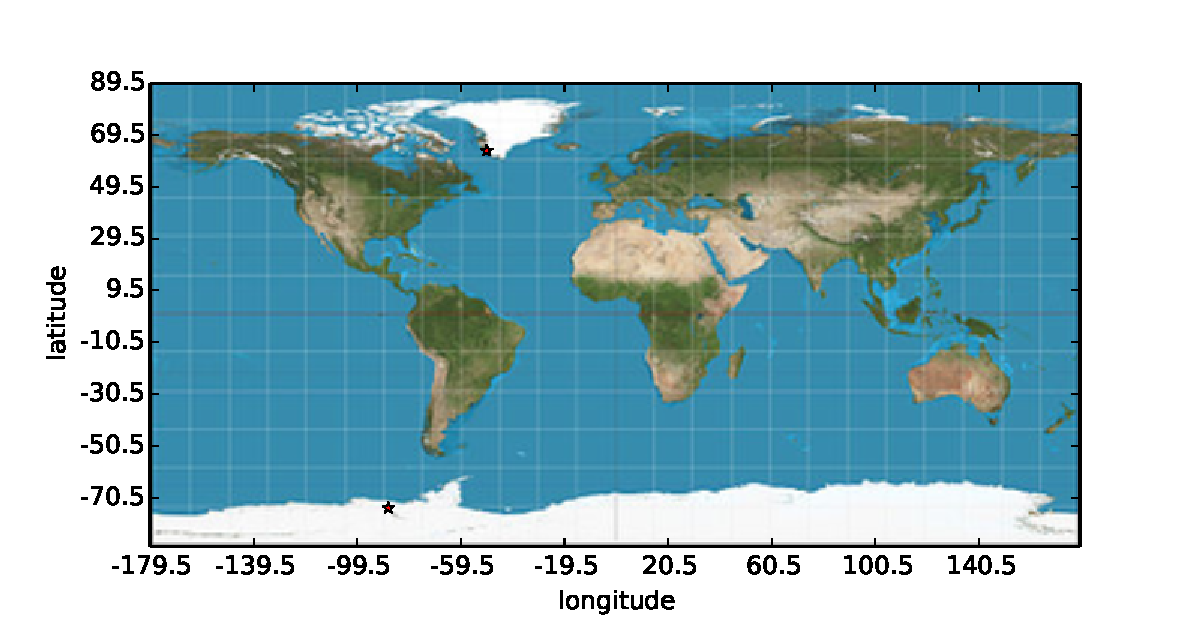
\includegraphics[height=6cm]{figures/ols-selected-map}
	\caption{The two selected locations, marked with a red star}
\end{figure}

\paragraph{Greenland}

At the west coast of Greenland is a strong period trend, caused by the the ice melting over the summer and reappearing over the winter. This trend is seen in Figure \ref{fig:ols-selected-0-fit}. In order to estimate the velocity and acceleration it's important that this trend is caught by the $\sin(\cdot)$ and $\cos(\cdot)$ terms in OLS regression.
\begin{figure}[H]
	\centering
	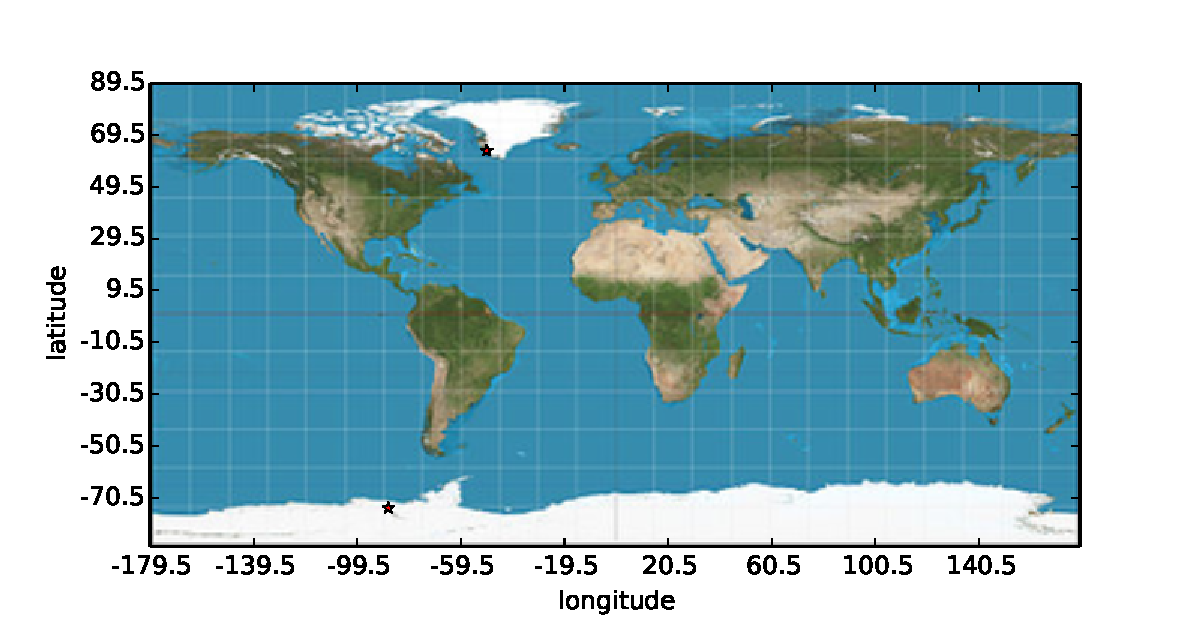
\includegraphics[width=\textwidth]{figures/ols-selected-0-fit}
	\caption{Messurements are blue, the OLS fit is red.}
	\label{fig:ols-selected-0-fit}
\end{figure}
 
From Figure \ref{fig:ols-selected-0-fit} it's seen that the period trend is caught by the model, however for some seasons (particular between 2008 and 2010) the fit is not very good. This is even more clear when looking at the residuals (Figure \ref{fig:ols-selected-0-residual}). From this it's clear that the residuals are far from white noise, which was one of the OLS assumptions.

\begin{figure}[H]
	\centering
	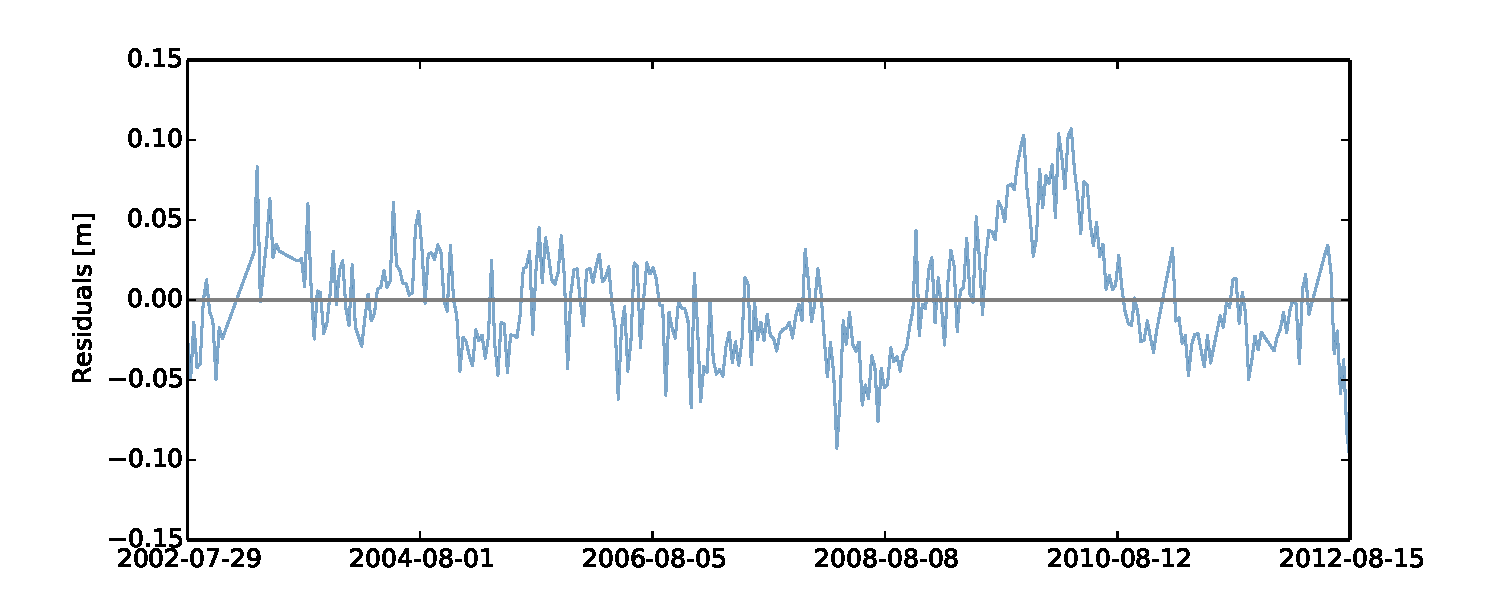
\includegraphics[width=\textwidth]{figures/ols-selected-0-residual}
	\caption{The OLS residuals are blue.}
	\label{fig:ols-selected-0-residual}
\end{figure}

%!TEX root=report.tex
\subsection{Reservations: Glacial Isostatic Adjustment}

The GRACE data that has been used in this report has not been corrected for Glacial Isostatic Adjustment (GIA) (sometimes also referred to as Post-glacial rebound) . 
GIA is an effect that makes land either rise, fall or shift horizontally. 
It can be observed at all locations which during the last ice age was covered by a thick layer of ice. 
The sheer weight of the ice compressed the crust of the Earth so much, that when the ice retracted and the downward force was removed the crust started to move.
 It is estimated that these movements will take many thousand years to subside. \\
Unfortunately the GRACE data does not adjust for the GIA effect.
 Thus it is impossible to know whether observed EWH patterns are actually mass losses/gains or just noise from GIA.
 Region specific averaging kernels are needed to properly account for GIA as well as noise from nearby land hydrology.
According to NASA \todo{insert source} the GRACE data is not suited for Cryospheric studies (ice mass changes) and thus one should keep these reservations in mind when viewing the results.

%!TEX root=report.tex

\subsection{Time series analysis - ARIMA}

To get an indication if its possible to use time series analysis on the GRACE data, a single position (63.5 N 49.5 W, west coast of Greenland) has been selected.

To analyze the data using an ARIMA model an equidistant dataset is required. For example it would otherwise not be possible to solve the Yule-Walker equations \cite[s.~122]{time-series-analysis}. In the original GRACE dataset some values are missing, thus they should be interpolated. Also in order to get an indication of the model performance, the last 36 observations (which corresponds to a year) have been separated for cross validation testing.

\begin{figure}[H]
\centering
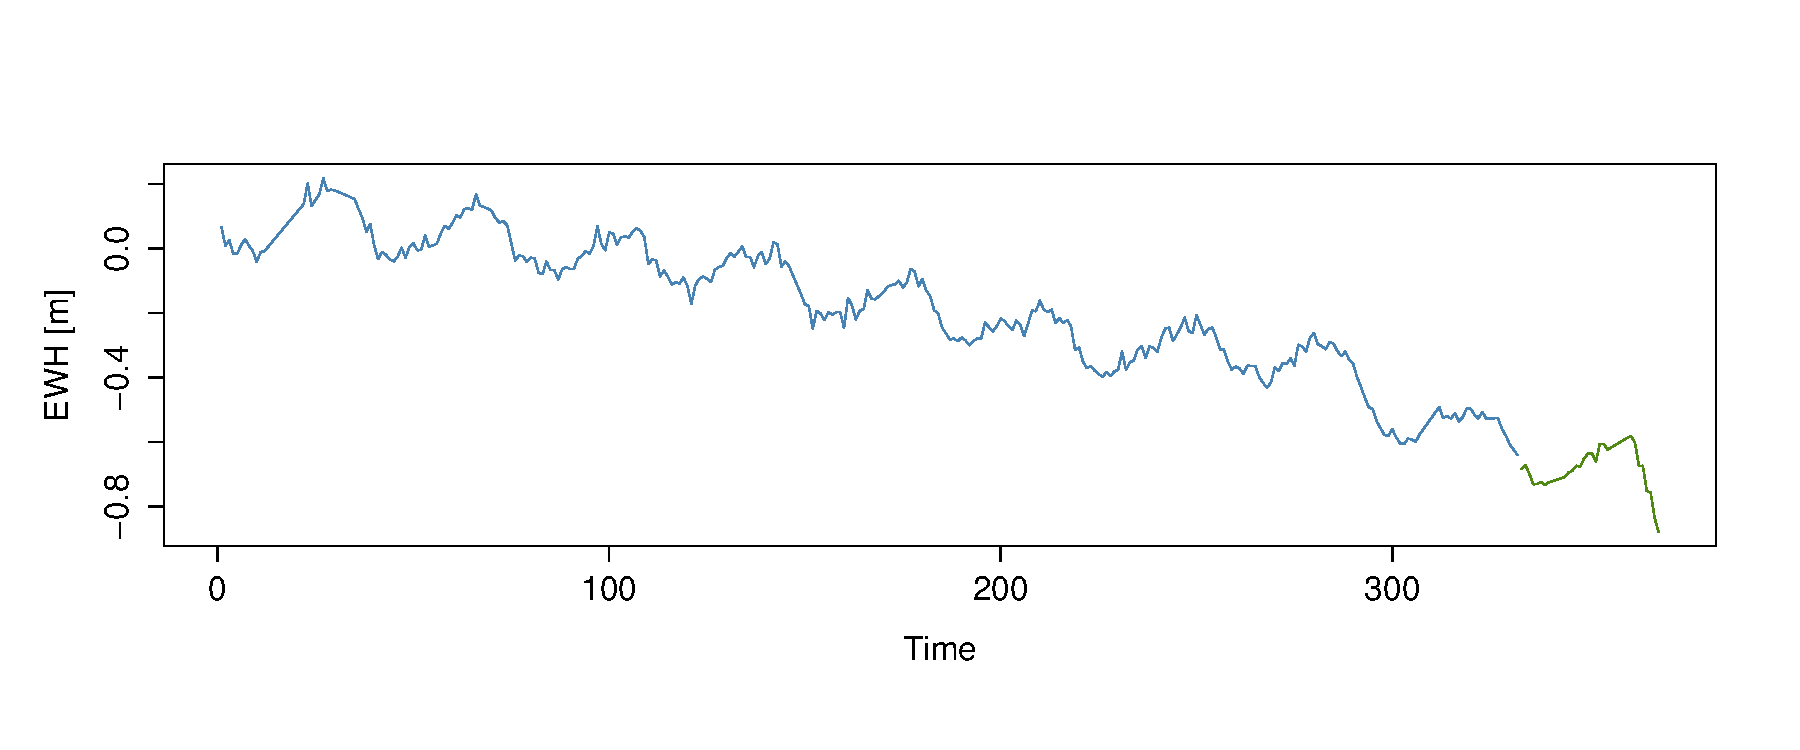
\includegraphics[height=5cm]{figures/ts-initial-split}
\caption{GRACE data at 63.5 N 49.5 W, where missing values are interpolated. Blue is the training data and green is the  test data.}
\label{fig:ts-initial-split}
\end{figure}

The time series in Figure \ref{fig:ts-initial-split} is clearly not stationary, thus it is necessary to consider the time series difference.
\begin{figure}[H]
\centering
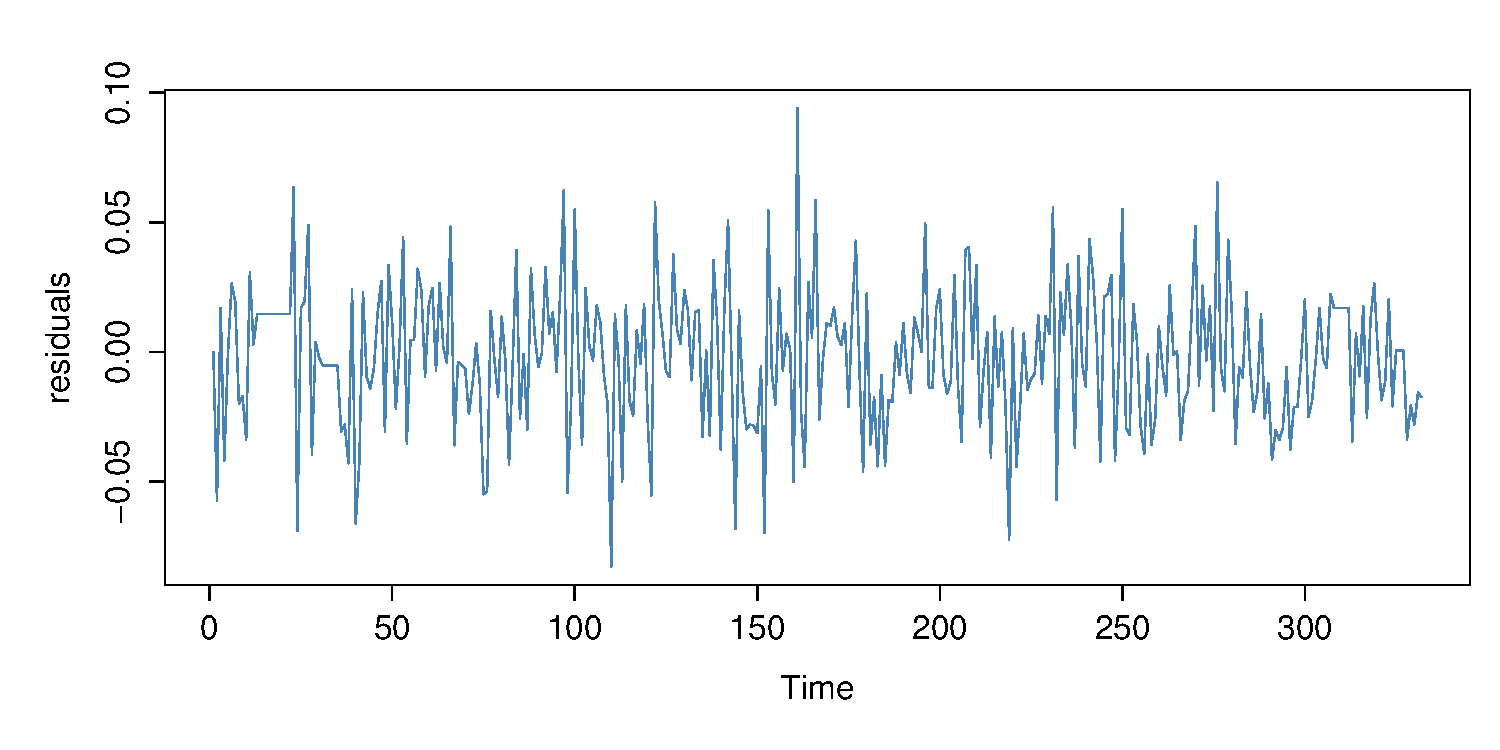
\includegraphics[height=5cm]{figures/ts-residual-i1s0}
\caption{The ARIMA$(0,1,0) \times (0,0,0)_{36}$ residuals.}
\label{fig:ts-residual-i1s0}
\end{figure}
On Figure \ref{fig:ts-residual-i1s0} there are some seasonal periods where the mean and variance are not the same as the remaining period, thus it is not completely stationary. Taking also the seasonal difference (assuming the season is 36 observations, a year) gives however a very stationary output.

\begin{figure}[H]
\centering
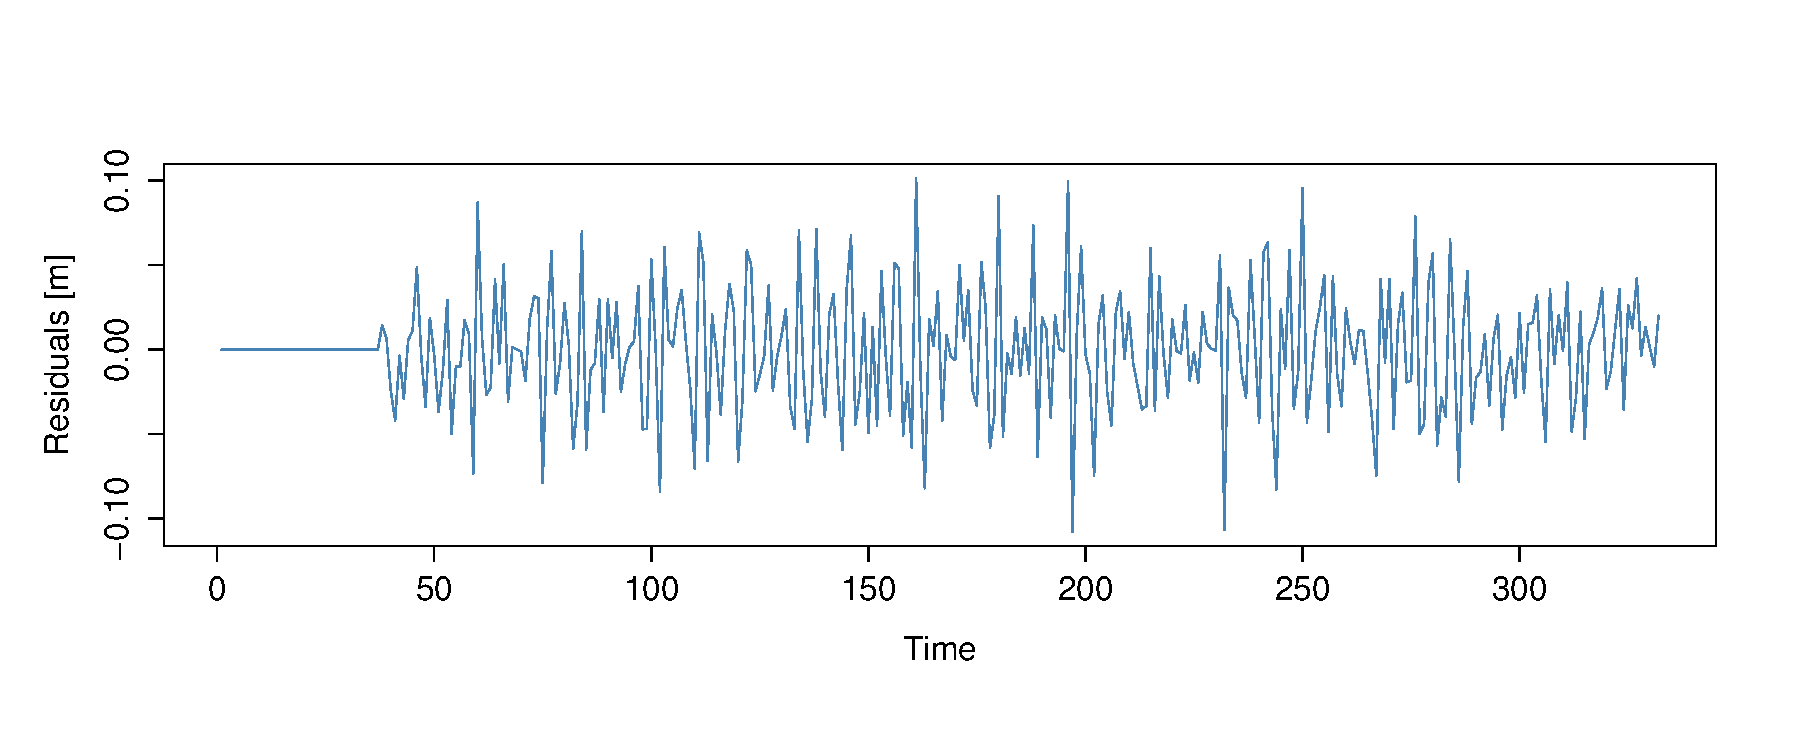
\includegraphics[height=5cm]{figures/ts-residual-i1s1}
\caption{The ARIMA$(0,1,0) \times (0,1,0)_{36}$ residuals.}
\label{fig:ts-residual-i1s1}
\end{figure}
On Figure \ref{fig:ts-residual-i1s1} its seen that the first 37 observations act strange, this is because there aren't enough past observations to estimate the EWH correctly, thus they should be excluded from further analysis.

To determine the AR and MA terms in the ARIMA model, the ACF and PACF should be estimated using the residuals from Figure \ref{fig:ts-residual-i1s1}.
\begin{figure}[H]
	\centering
	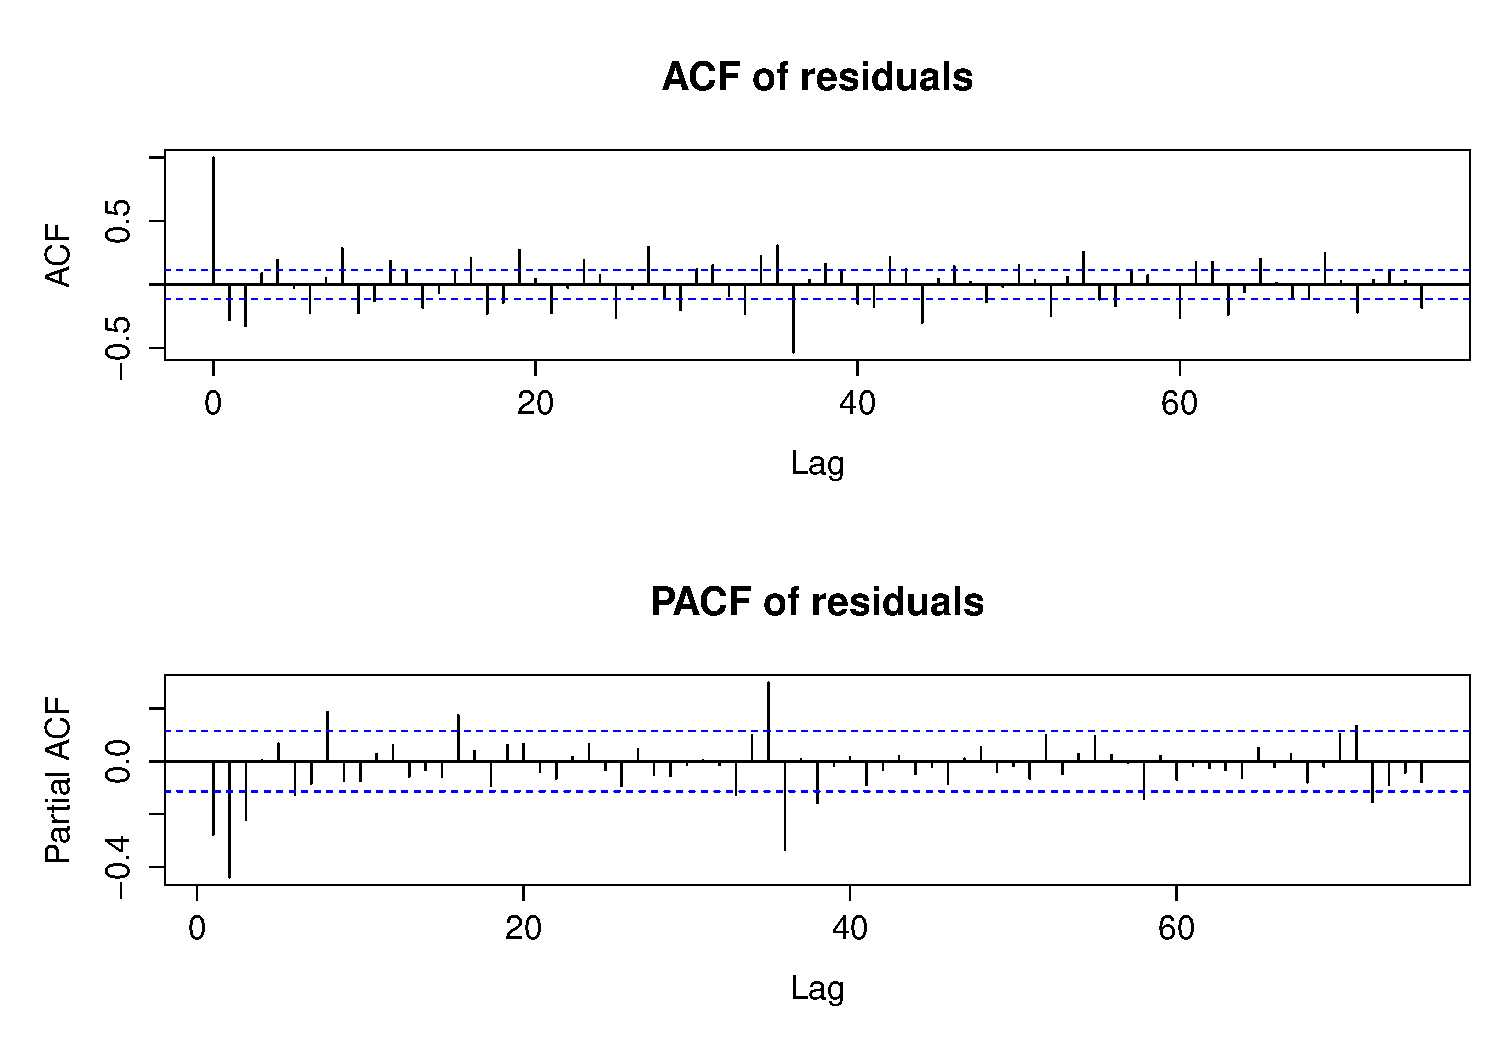
\includegraphics[width=\textwidth]{figures/ts-acf-ar0s0}
	\caption{ACF and PACF for ARIMA$(0,1,0) \times (0,1,0)_{36}$ residuals}
	\label{fig:ts-acf-ar0s0}
\end{figure}

Using the PACF in Figure \ref{fig:ts-acf-ar0s0} and the rules for the AR term \cite[Table~6.1]{time-series-analysis} \texttt{AR(2)}, seams like a good guess for the non-seasonal AR term.
\begin{figure}[H]
	\centering
	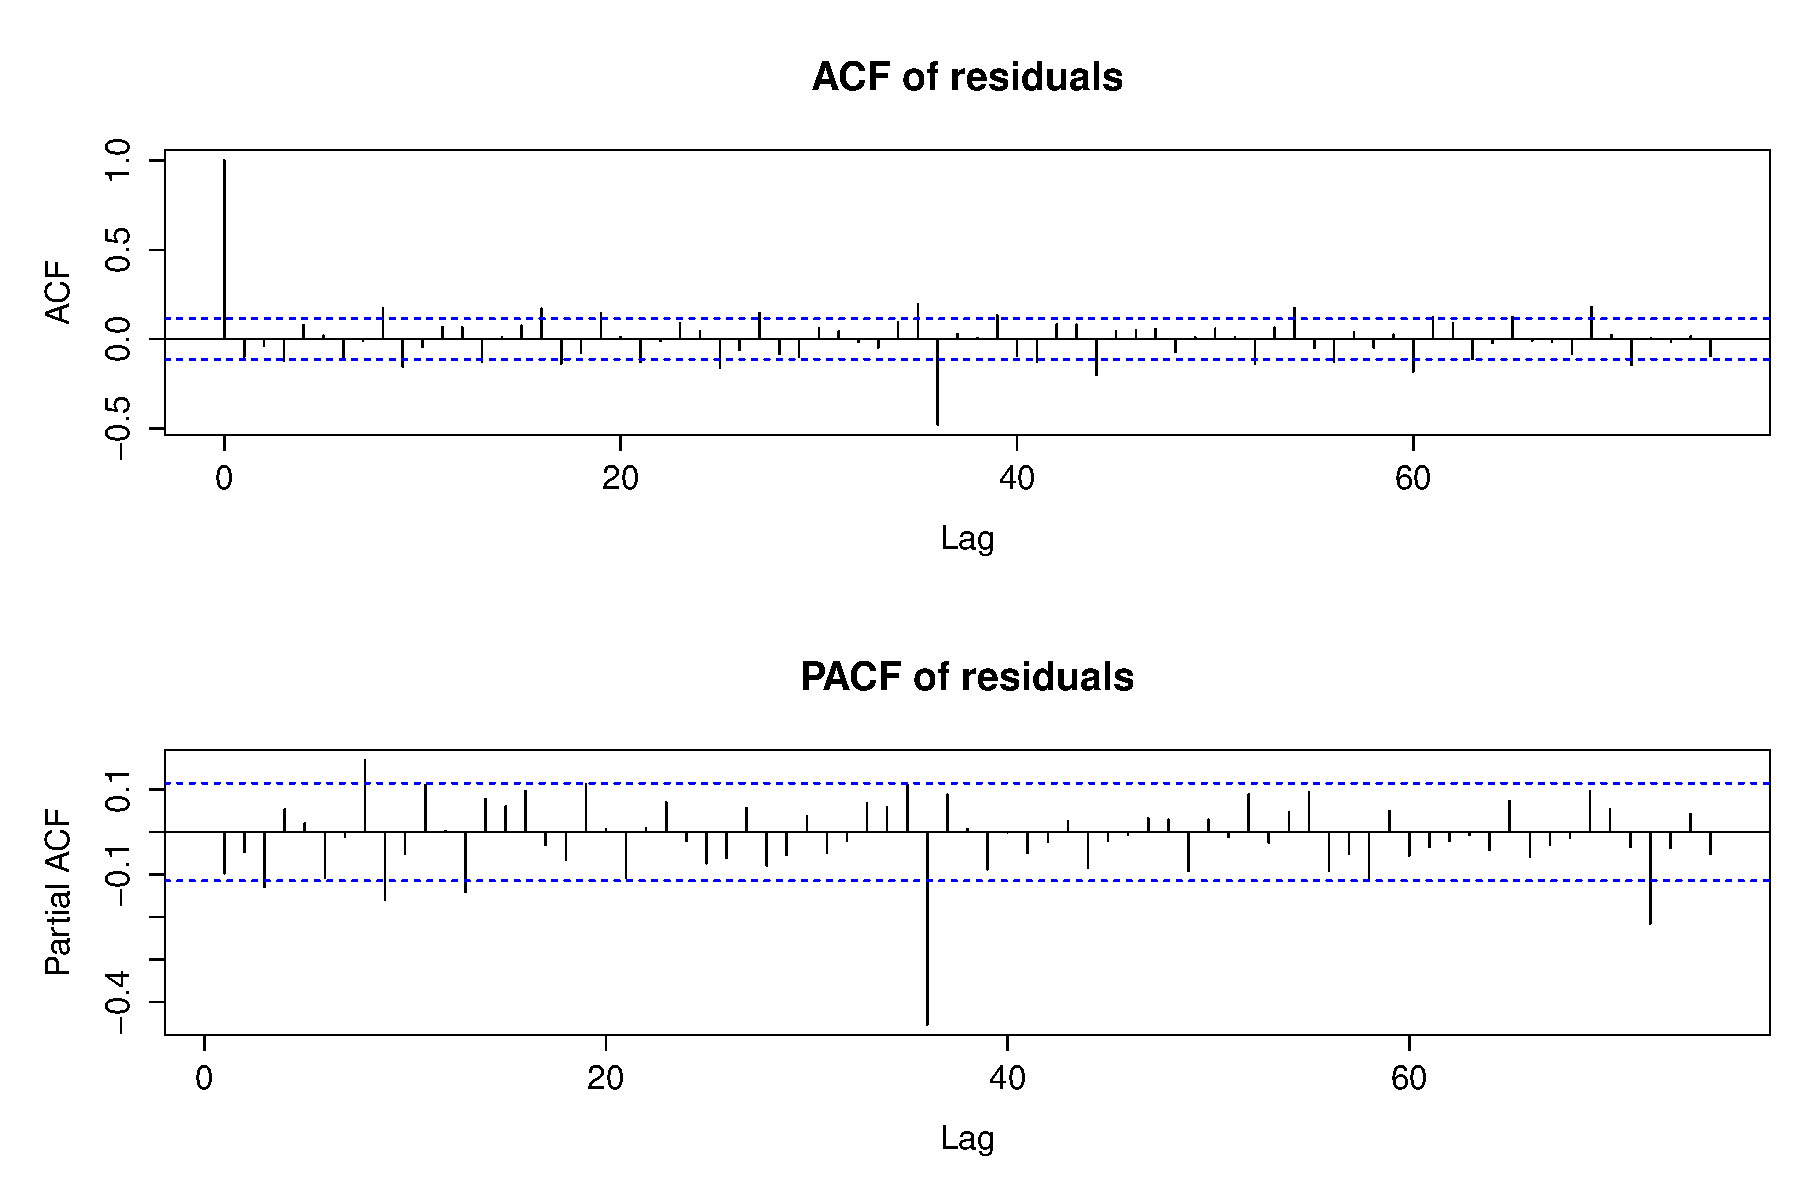
\includegraphics[width=\textwidth]{figures/ts-acf-ar2s0}
	\caption{ACF and PACF for ARIMA$(2,1,0) \times (0,1,0)_{36}$ residuals}
	\label{fig:ts-acf-ar2s0}
\end{figure}

This clearly fitted the non-seasonal trend. From Figure \ref{fig:ts-acf-ar0s0} it might have looked like there was a \texttt{AR(3)} or \texttt{MA(2)} term, but the \texttt{AR(2)} is the simplest of those and fit the trend just fine. The seasonal part is now extremely apparent in Figure \ref{fig:ts-acf-ar2s0}, where it looks like either a \texttt{SAR(2)}- or a \texttt{SAR(1)}-term.
\begin{figure}[H]
	\centering
	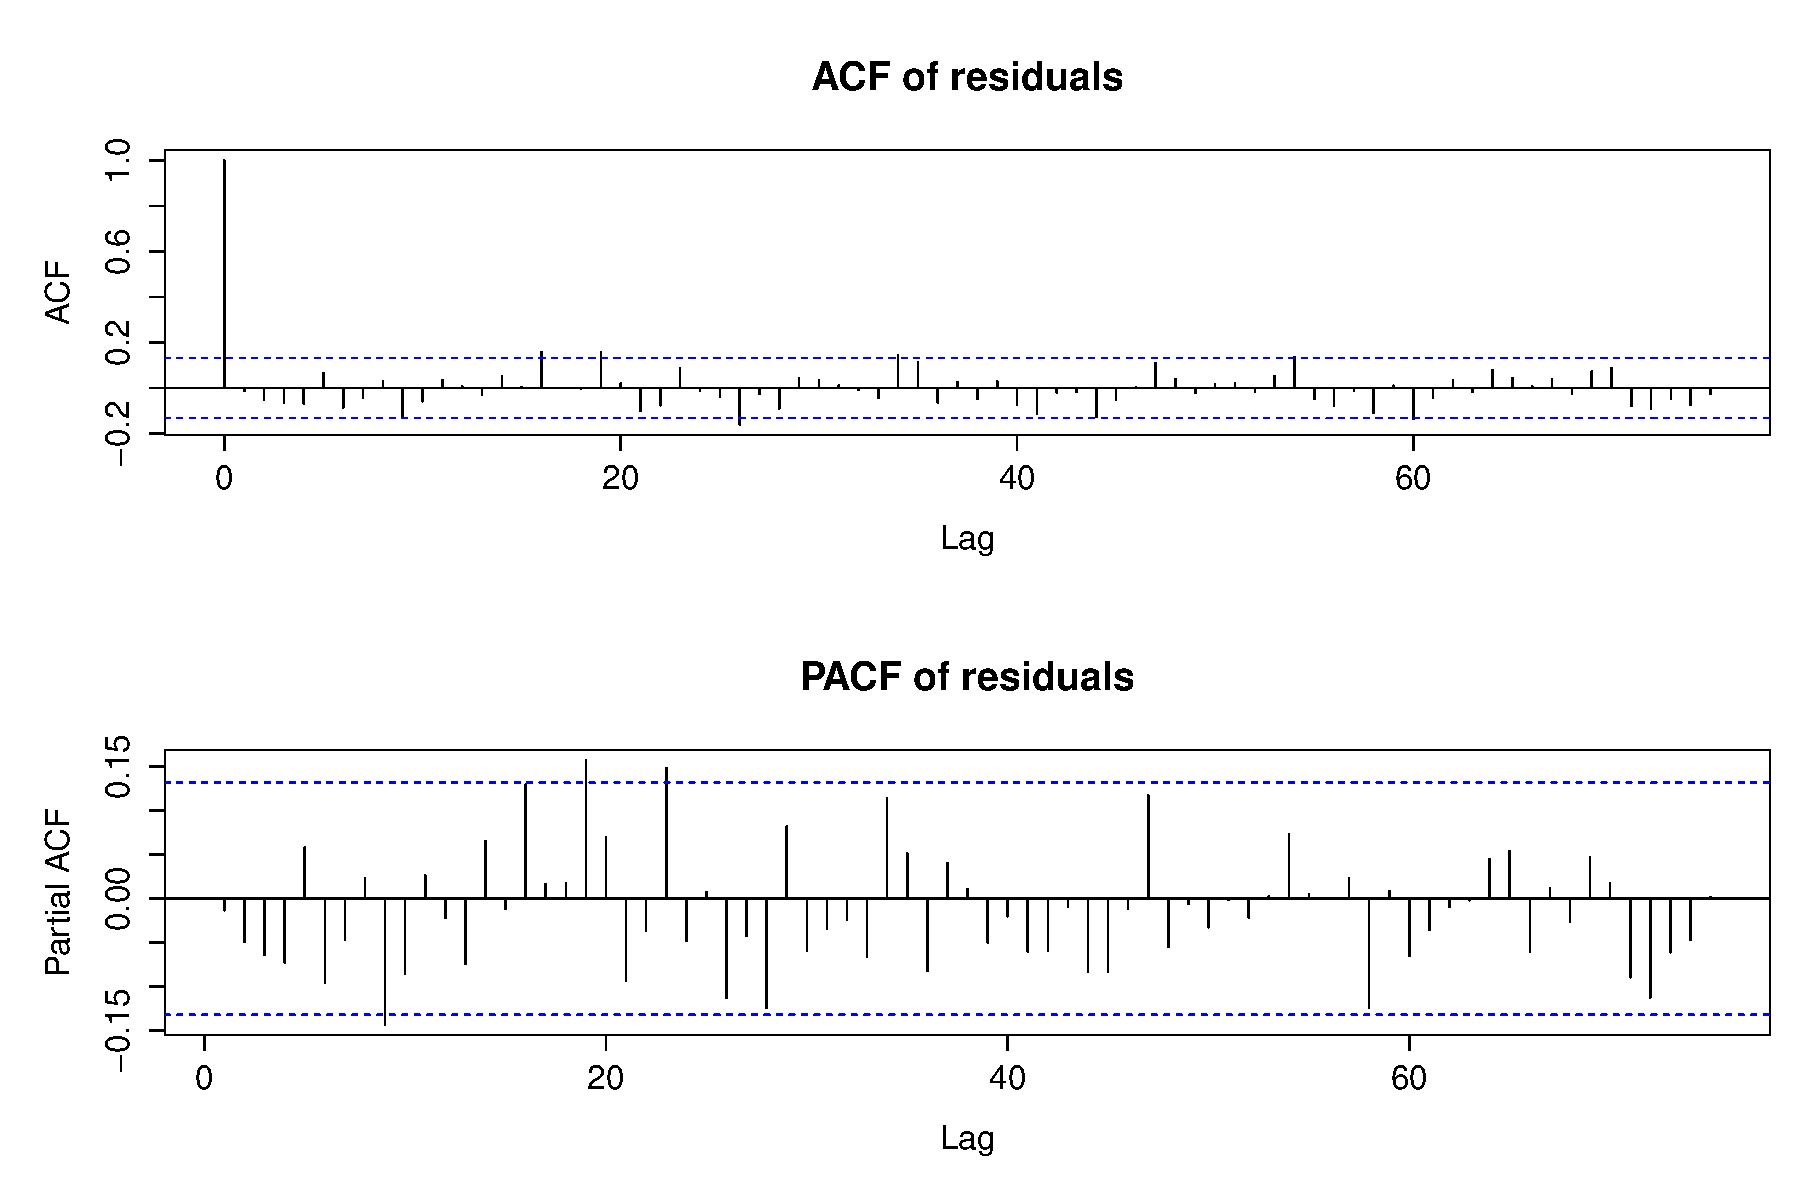
\includegraphics[width=\textwidth]{figures/ts-acf-ar2s2}
	\caption{ACF and PACF for ARIMA$(2,1,0) \times (2,1,0)_{36}$ residuals}
	\label{fig:ts-acf-ar2s2}
\end{figure}

From just looking at the estimated ACF and PACF in Figure \ref{fig:ts-acf-ar2s2}, ARIMA$(2,1,0) \times (2,1,0)_{36}$ seems like a good choice. To finally validate the model, a good start is to look at the residuals.
\begin{figure}[H]
	\centering
	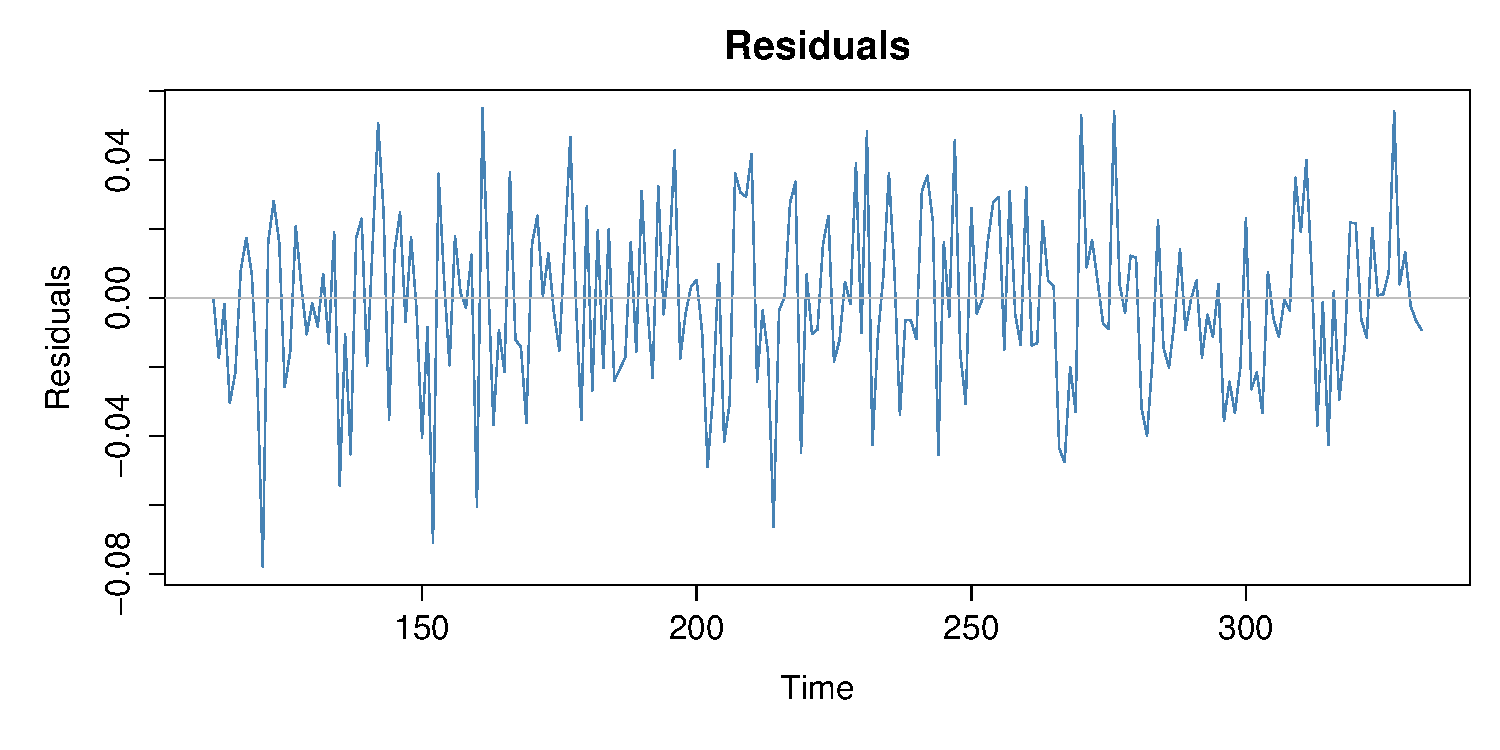
\includegraphics[height=5cm]{figures/ts-final-residual}
	\caption{ARIMA$(2,1,0) \times (2,1,0)_{36}$ residuals. The first 111 residuals have been skipped since they cannot be estimated correctly.}
	\label{fig:ts-final-residual}
\end{figure}

Figure \ref{fig:ts-final-residual} looks stationary, there are no outliers nor seasonal trends. To validate the model further the Ljung-Box test can be used. This however requires the residuals to be normally distributed, a QQ-plot (Figure \ref{fig:ts-final-qq}) shows that this is the case:
\begin{figure}[H]
	\centering
	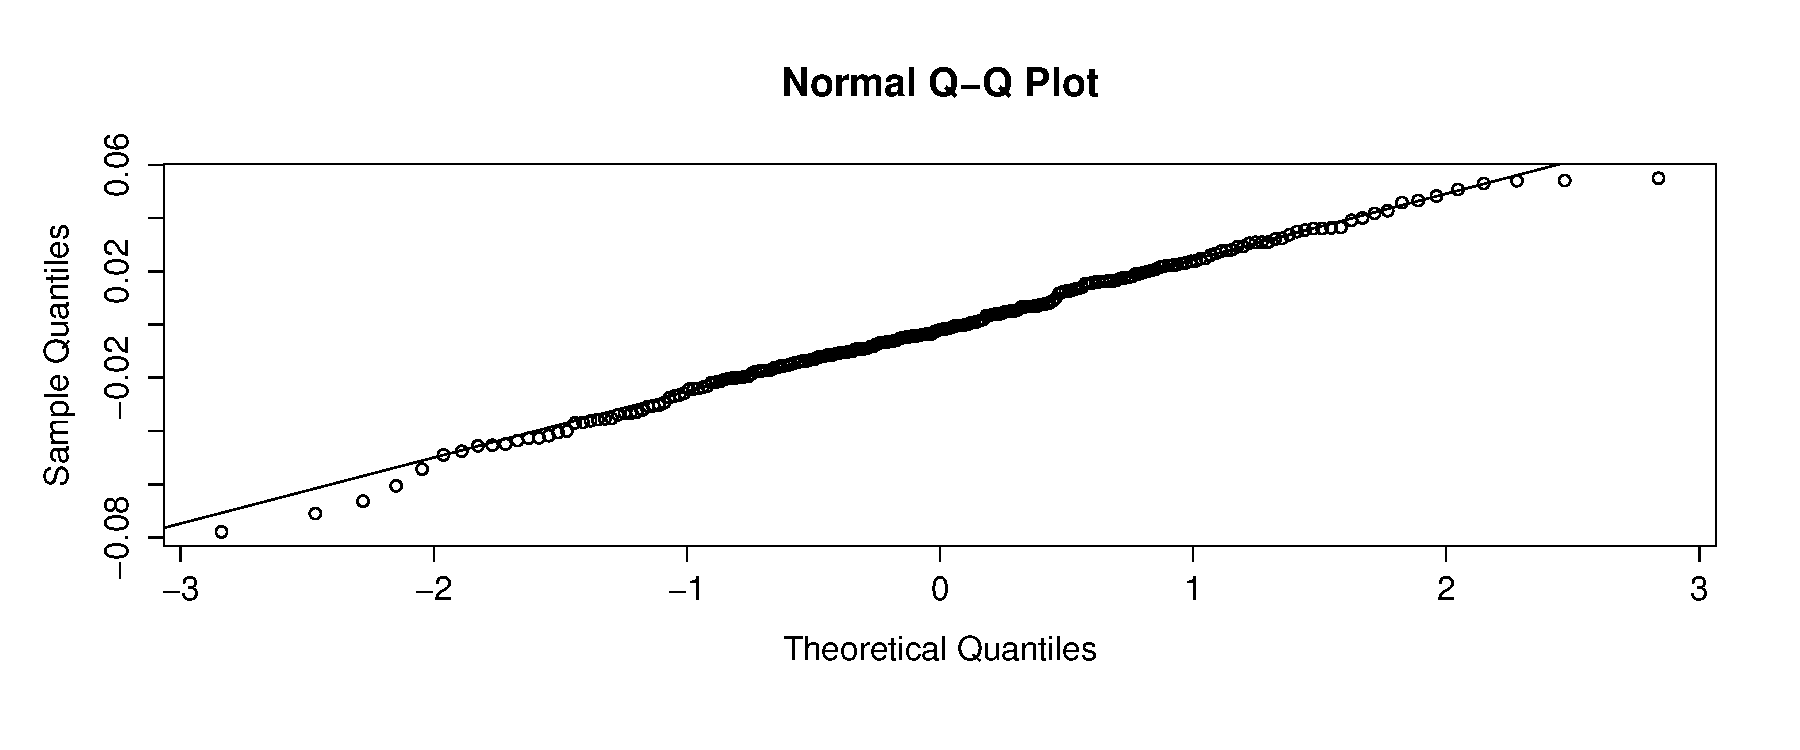
\includegraphics[height=5cm]{figures/ts-final-qq}
	\caption{QQ-plot for the ARIMA$(2,1,0) \times (2,1,0)_{36}$ residuals.}
	\label{fig:ts-final-qq}
\end{figure}

\begin{figure}[H]
	\centering
	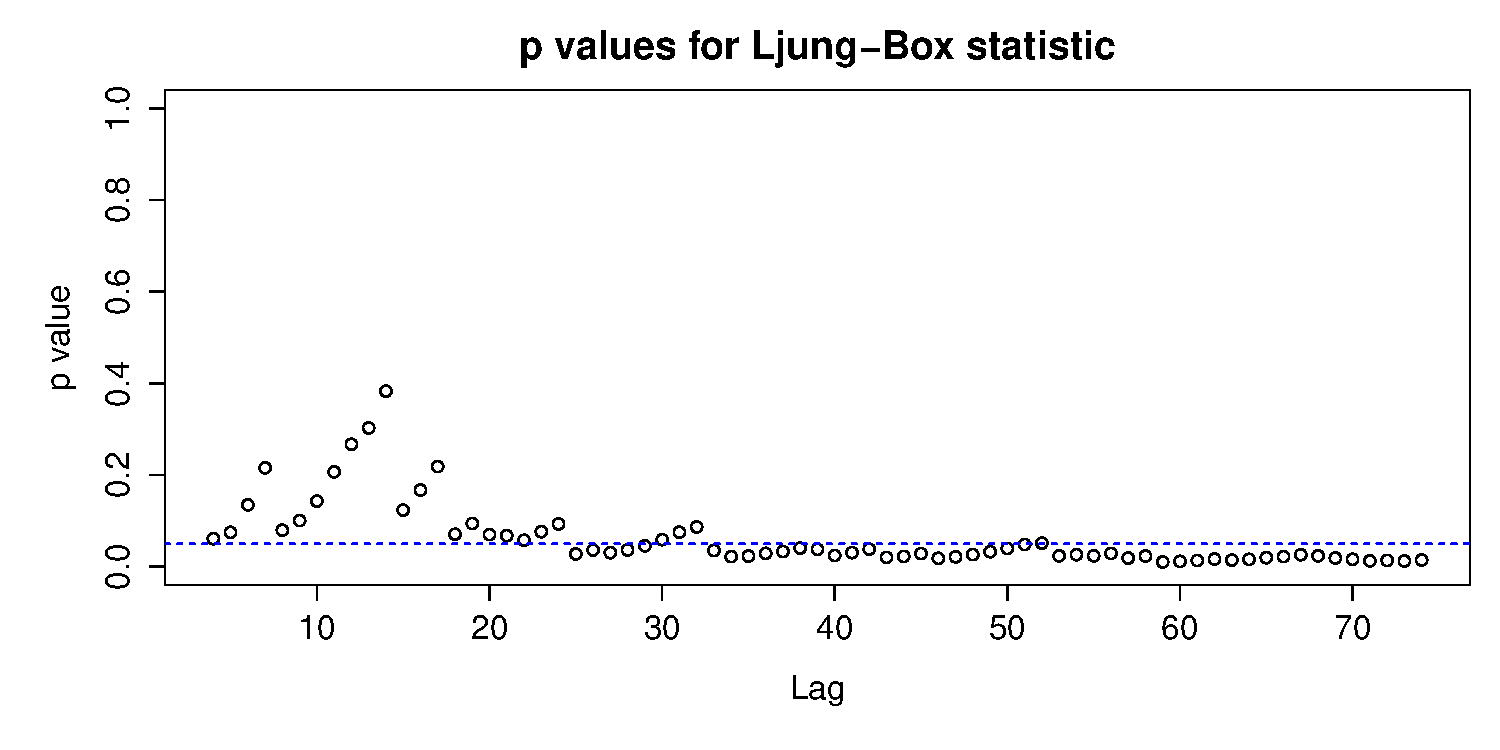
\includegraphics[height=5cm]{figures/ts-final-ljungbox}
	\caption{Ljung-Box test for the ARIMA$(2,1,0) \times (2,1,0)_{36}$ residuals.}
	\label{fig:ts-final-ljungbox}
\end{figure}

From the Ljung-Box test (Figure \ref{fig:ts-final-ljungbox}) the p-value for the first many lags looks good, however after 25 it can be with 95\% confidence statically significant concluded that the residuals are correlated. In terms of pure time series analysis is makes the model quite useless, however it is still valuable to do the cross validation.

\begin{figure}[H]
\centering
\centerline{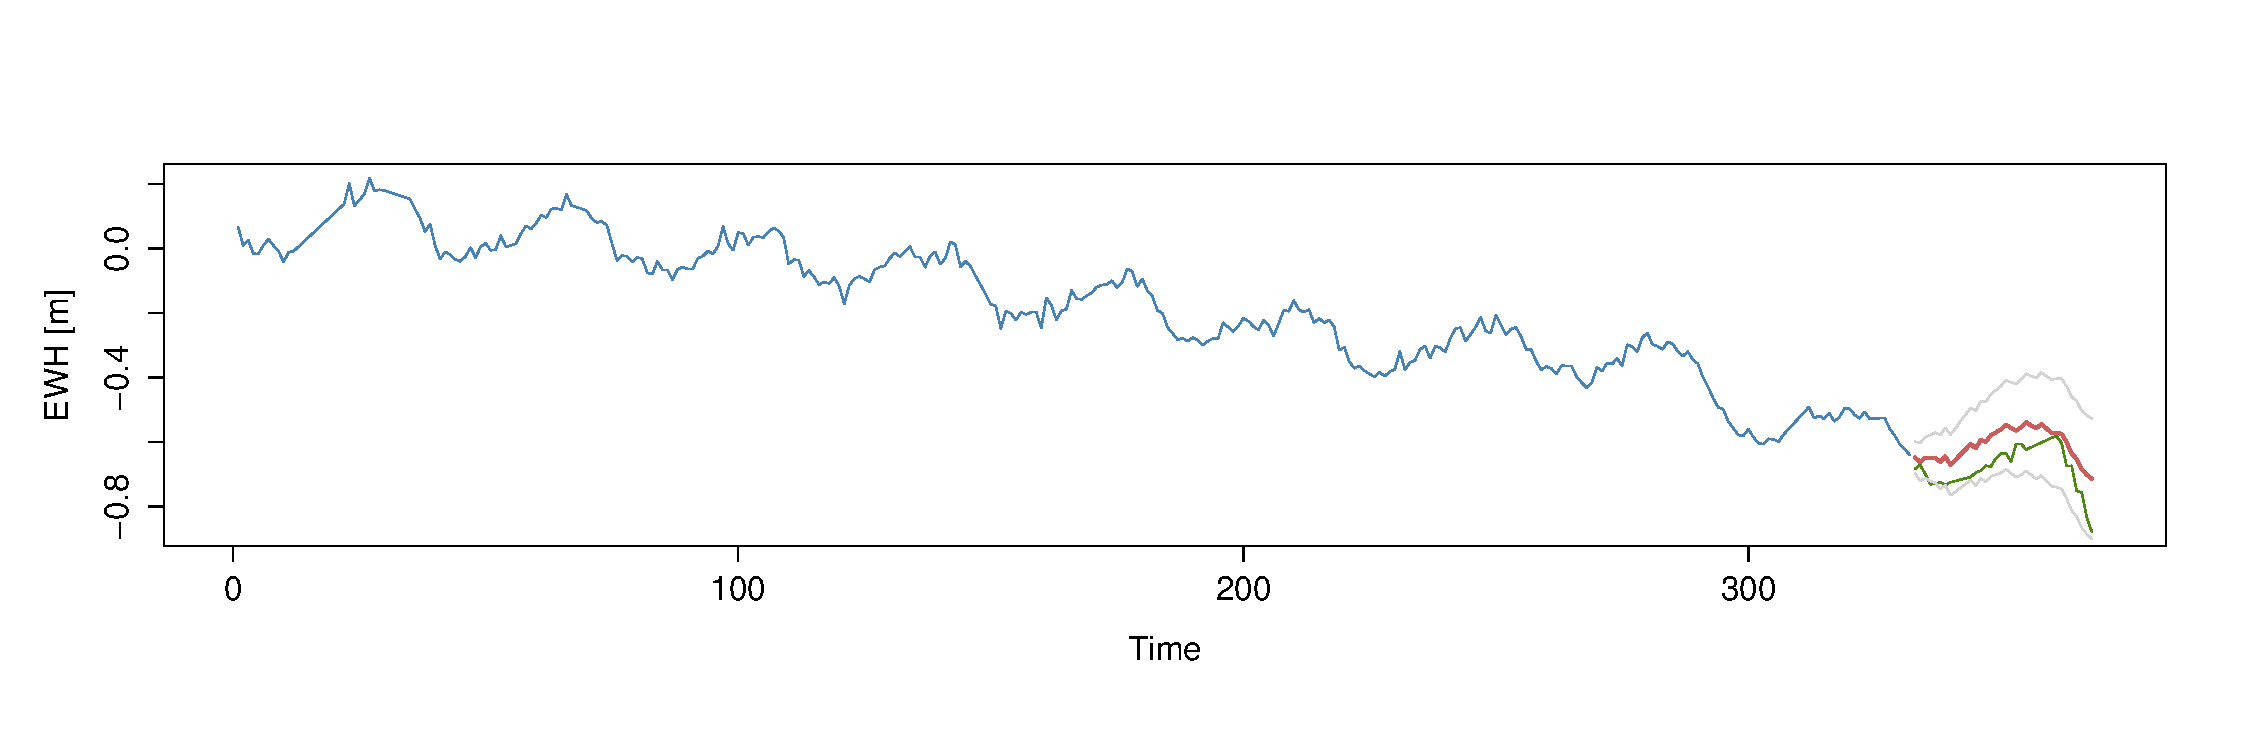
\includegraphics[height=6cm]{figures/ts-final-forecast}}
\caption{Forecast on Cross Validation. Blue is the training data, green is the test data. Red is then the predicted test values with its 95\% confidence interval marked with gray lines.}
\label{fig:ts-final-forecast}
\end{figure}

From Figure \ref{fig:ts-final-forecast} it quite clear that the test data is consistently bellow the expectation line (red). While it is still inside the 95\% confidence interval, this high correlation in the error between lags indicates that the model is not particular useful. 

%!TEX root=report.tex
\pagebreak
\subsection{Least angular regression (LAR)}

The full solution path is in this case very hard to interpret, so instead the relative coefficients are shown. That is the coefficients at an iteration divided by the final value (the plain OLS case).

\begin{figure}[H]
	\centering
	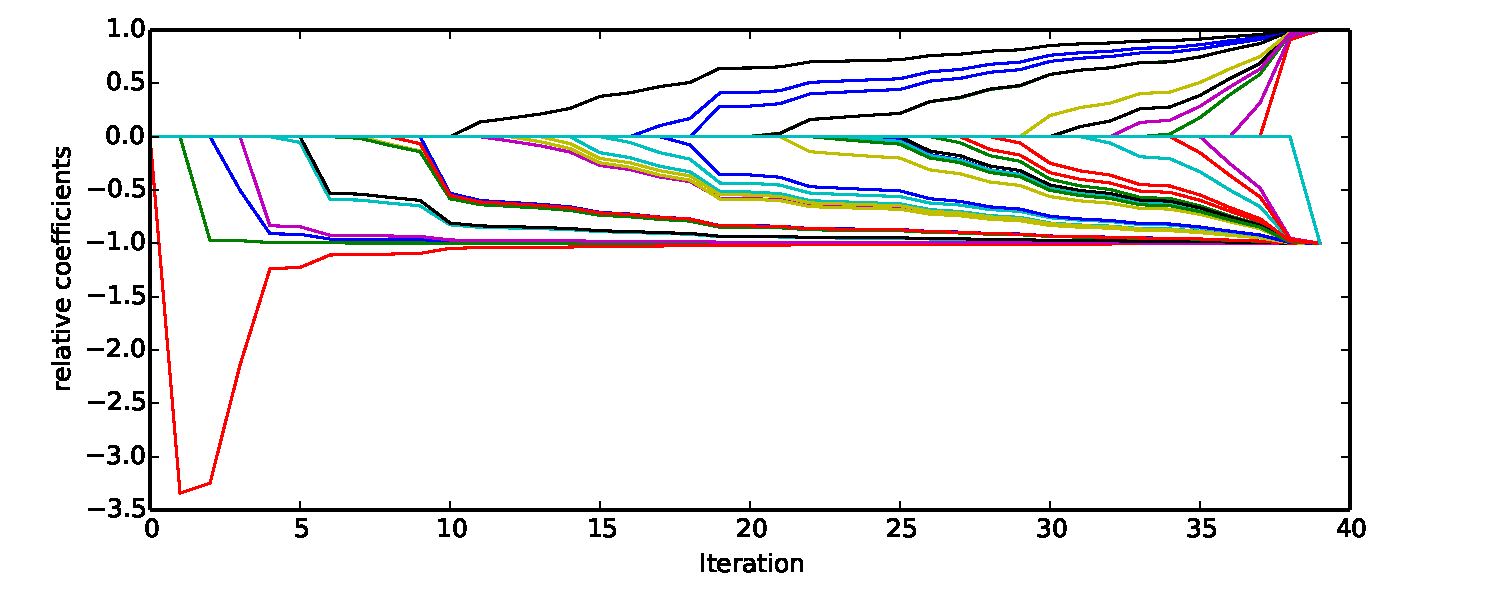
\includegraphics[width=\textwidth]{figures/lar-coefficients}
	\caption{The full solution path shown with relative coefficients. Position is 63.5 N 49.5 W, west coast of Greenland.}
	\label{fig:lar-coefficients}
\end{figure}

From Figure \ref{fig:lar-coefficients} it appears that the first 7 coefficients are the more relevant. 
\begin{table}[H]
\centering
\begin{tabular}{r|l}
name                 & coeffecients \\ \hline
intercept ($1$) & $-1.69 \cdot 10^{-1}[m]$ \\
velocity ($t$) & $-2.23 \cdot 10^{-4} [\sfrac{m}{day}]$ \\
acceleration ($0.5 \cdot t^2$) & $-9.16 \cdot 10^{-8} [\sfrac{m}{day^2}] $ \\
$\cos(2 \pi /365.2 * t)$ & $-8.06 \cdot 10^{-3}$ \\
$\sin(2 \pi /365.2 * t)$ & $-7.67 \cdot 10^{-2}$ \\
$\sin(2 \pi /182.6 * t)$ & $-7.59 \cdot 10^{-3}$ \\
$\sin(2 \pi /121.7 * t)$ & $-8.67 \cdot 10^{-5}$
\end{tabular}
\caption{LAR coefficients in the seventh iteration}
\end{table}

Using these seven coefficients the following line $\hat{y}$ can be calculated:
\begin{figure}[H]
\center
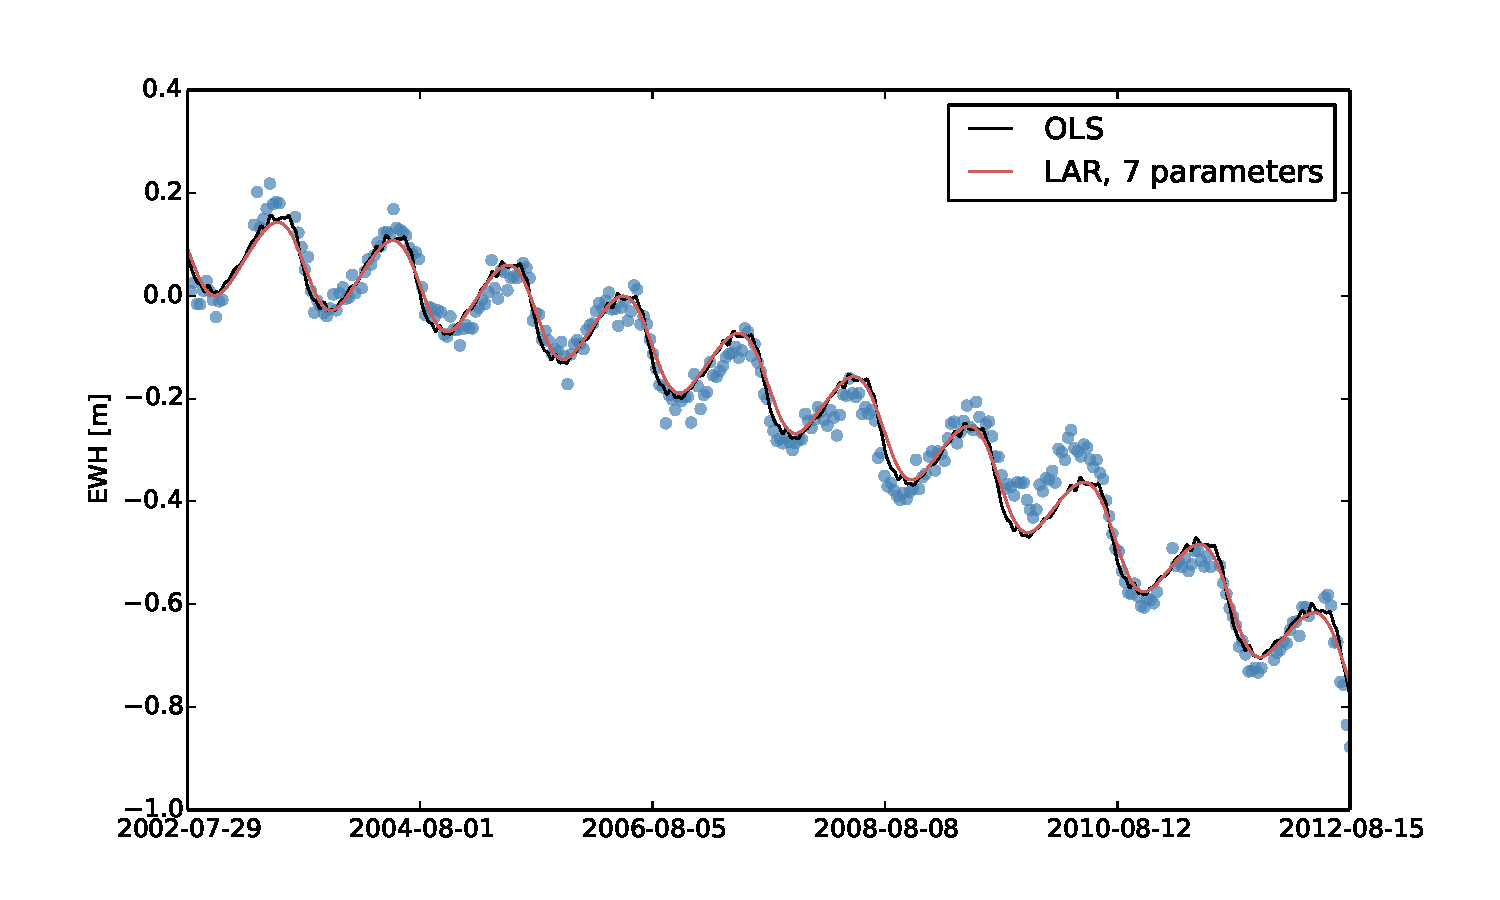
\includegraphics[width=\textwidth]{figures/lar-compare}
\caption{OlLS and LAR (seven parameters) compared. Position is 63.5 N 49.5 W, west coast of Greenland.}
\end{figure}

\subsubsection{How many frequencies are actually needed}

This was done for one position on the globe only. If one were to apply this to other positions one might get different lasso-paths and perhaps also a slight variation in the number of coefficients needed. For example for modeling the ocean one would not need as many coefficients, while at places with heavy rain season such as South America, more coefficients might be needed.

%!TEX root=report.tex

\subsection{OLS AR(1)}
The difference between standard OLS and the proposed model for OLS with autocorrelated residuals was examined for a multitude of different locations on the globe.
Now, since the AR part of the model requires equidistant time series a linear interpolation was used to fill in the many gaps that existed in the data. 
Sadly, however, even when using interpolated time series there seemed to be very little difference between the two models. This was a bit surprising since the $\rho$ estimate almost always was close to $0.9$ and in some cases even higher. 

Since the difference between models were negligible, we find that it suffices to show the results for just one such location (in this case (lon,lat)$=(24,134)$).
Firstly a visual representation of the differences:

\begin{figure}[H]
\centering
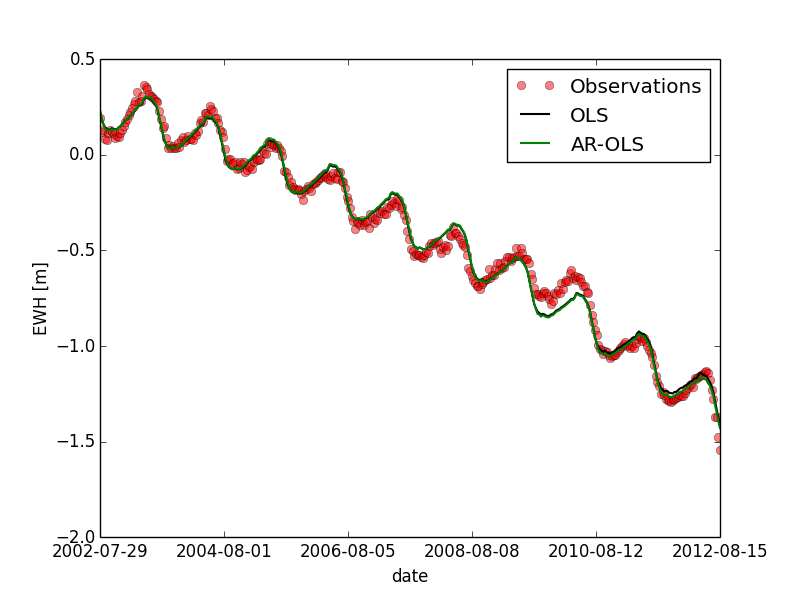
\includegraphics[width=1.0\linewidth]{figures/ols-AR(1)-24-134}
\caption{OLS. vs OLS with autocorrrelated residuals - comparison made for the west coast of Greenland. Here $\hat{\rho}\approx0.894$.}
\end{figure}

Secondly, follows an overview of the models:
\begin{tabular}{l || c |  r}[H]
 & OLS & OLS-AR(1) \\ \hline
$R^2$ & 0.990 &0.875 \\
AIC & -1149 &-1742 \\
Durbin-Watson & 0.208 & 2.354
\end{tabular}\\\\
On the positive side the Durbin-Watson test suggest that the model improved  ($0\ge D\ge 4$. $D<<2$ implies positive autocorrelation between the residuals while $D>>2$ implies negative autocorrelation). 
As discussed in the theory section, when $D<<2$ model estimates tend to be too optimistic.
 This is seen in the table above as well as in the estimated t-scores (not shown here). 
\\
Seeing as the OLS overestimates its performance and the model predictions look visually similar(this is due to the fact that the biggest absolute difference in $\beta$ coefficients is $10^-3$) it is hard to objectively identify the best model.
 However, if one were pressed to conclude something it might be that the OLS-AR(1) model most likely provides a more realistic estimate of the model performance than pure OLS. 
So to recap, the $\beta$-vector estimates were found to be almost identical and the only improvement offered by OLS-AR(1) is given by more precise p-values.

%!TEX root=report.tex
\subsection{Splines}
Using 9 knots with a year in between and letting the sine and cosine function enter at each knot, one can allow for different seasons. The columns in $X$ can be visualized as in Figure \ref{fig:splines-x-columns}.
\begin{figure}[H]
	\centering
	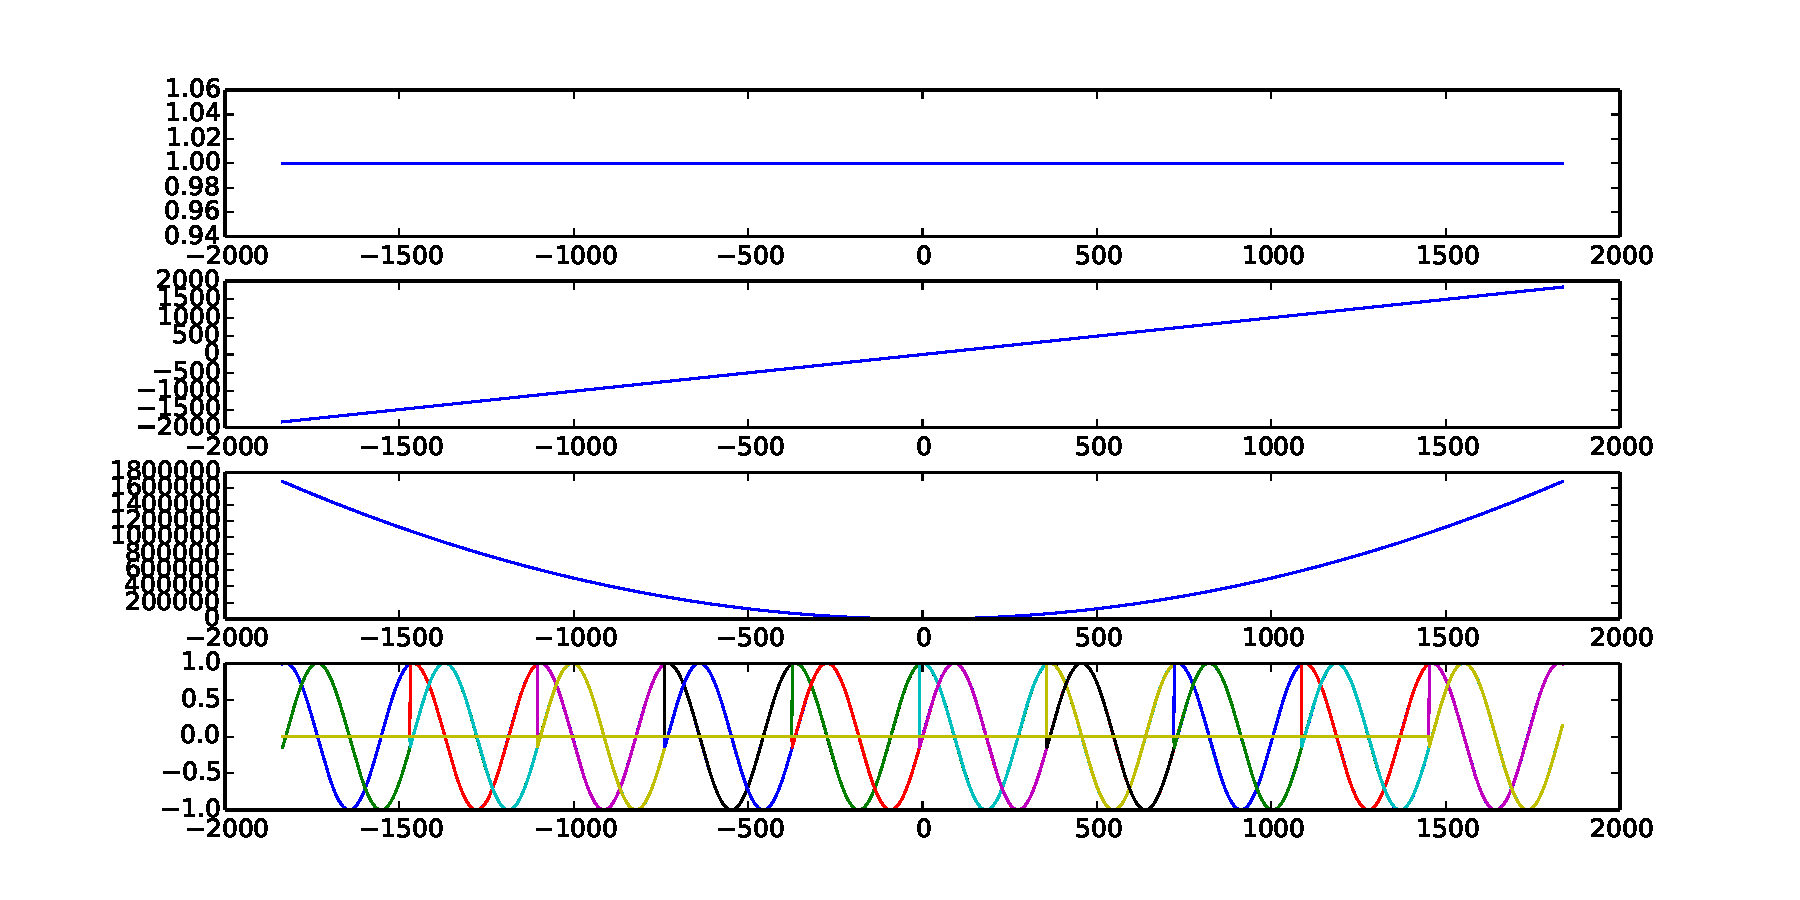
\includegraphics[width=\textwidth]{figures/splines-x-columns}
	\caption{Constant, trend and acceleration in the 3 uppermost plots. Sine and cosine hinge functions in the bottom plot.}
	\label{fig:splines-x-columns}
\end{figure}

A RMSE diagnostic shows that the residuals are indeed smaller (max standard OLS was 0.135).

\begin{figure}[H]
	\centering
	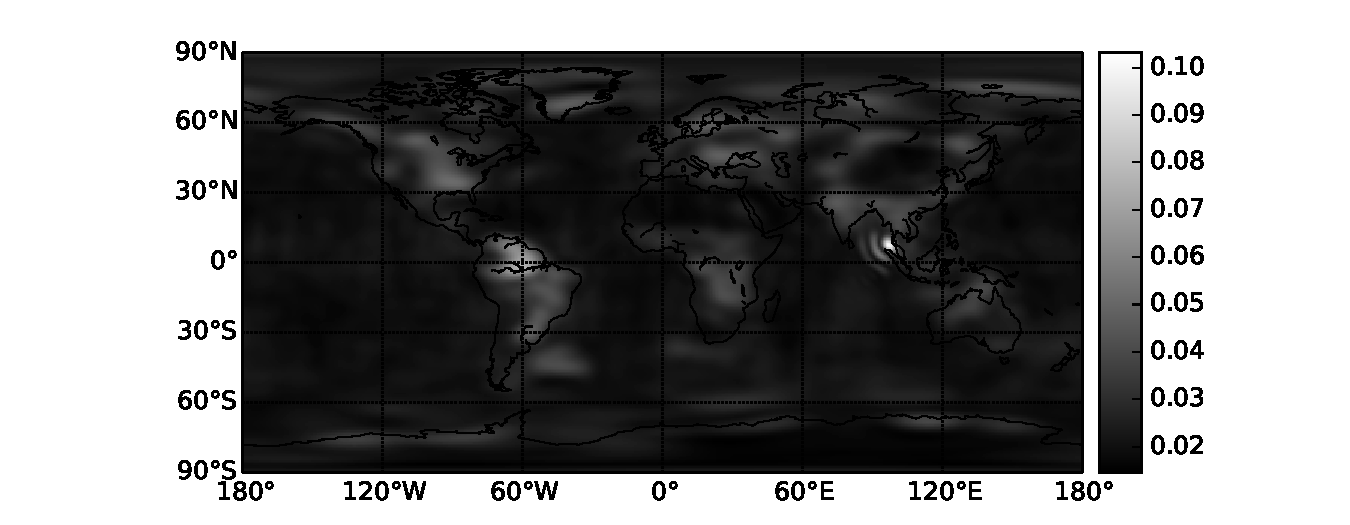
\includegraphics[width=\textwidth]{figures/splines-rmse}
	\caption{RMSE for each position using basis expansion.}
	\label{fig:splines-rmse}
\end{figure}

Looking at the west coast of Greenland now using a basis expansion, the overall fit (Figure \ref{fig:splines-selected-0-fit}) looks improved. For some reason 2009 still causes some issues, which is partially seen in the residuals (Figure \label{fig:splines-selected-0-residual}). Another thing to notices is that the curves are a lot more smooth, but this is simply because only the first 3 frequencies (year, half year and quarter year) was used. This was to prevent the degrees of freedom to drop dramatically, dude to the otherwise huge amount of parameters.
\begin{figure}[H]
	\centering
	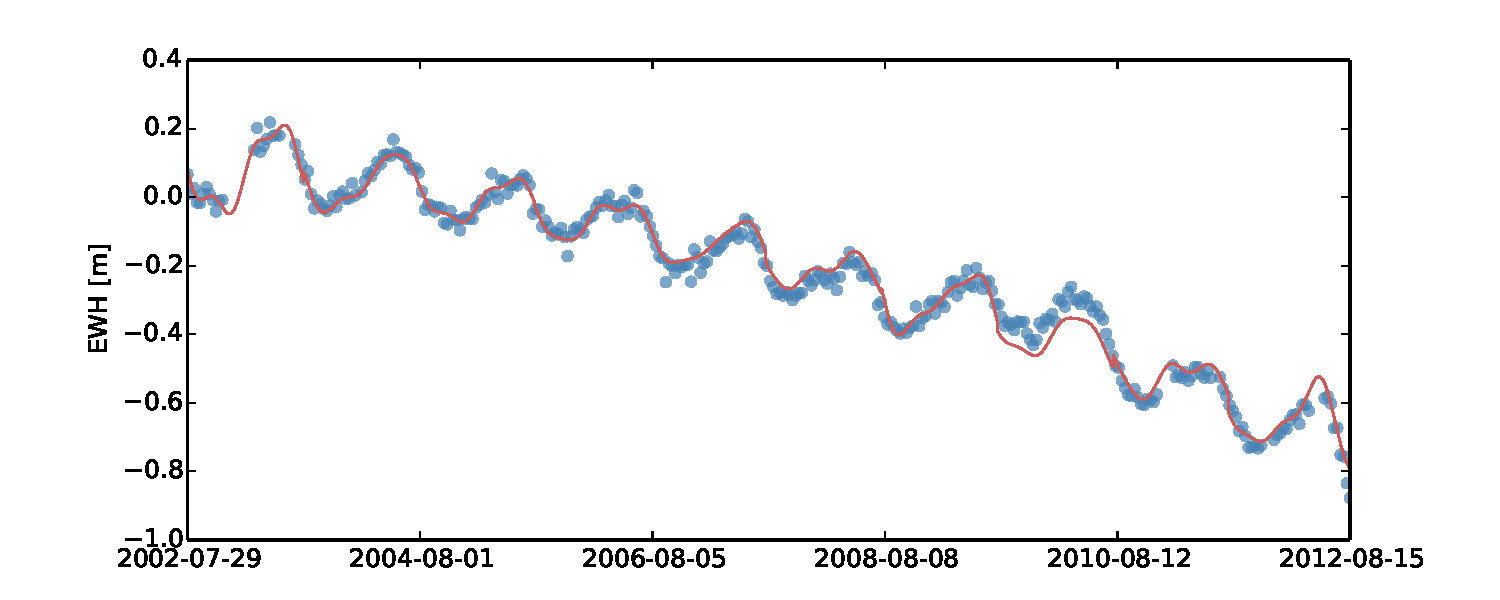
\includegraphics[width=\textwidth]{figures/splines-selected-0-fit}
	\caption{Measurements are blue, the OLS fit is red.}
	\label{fig:splines-selected-0-fit}
\end{figure}

\begin{figure}[H]
	\centering
	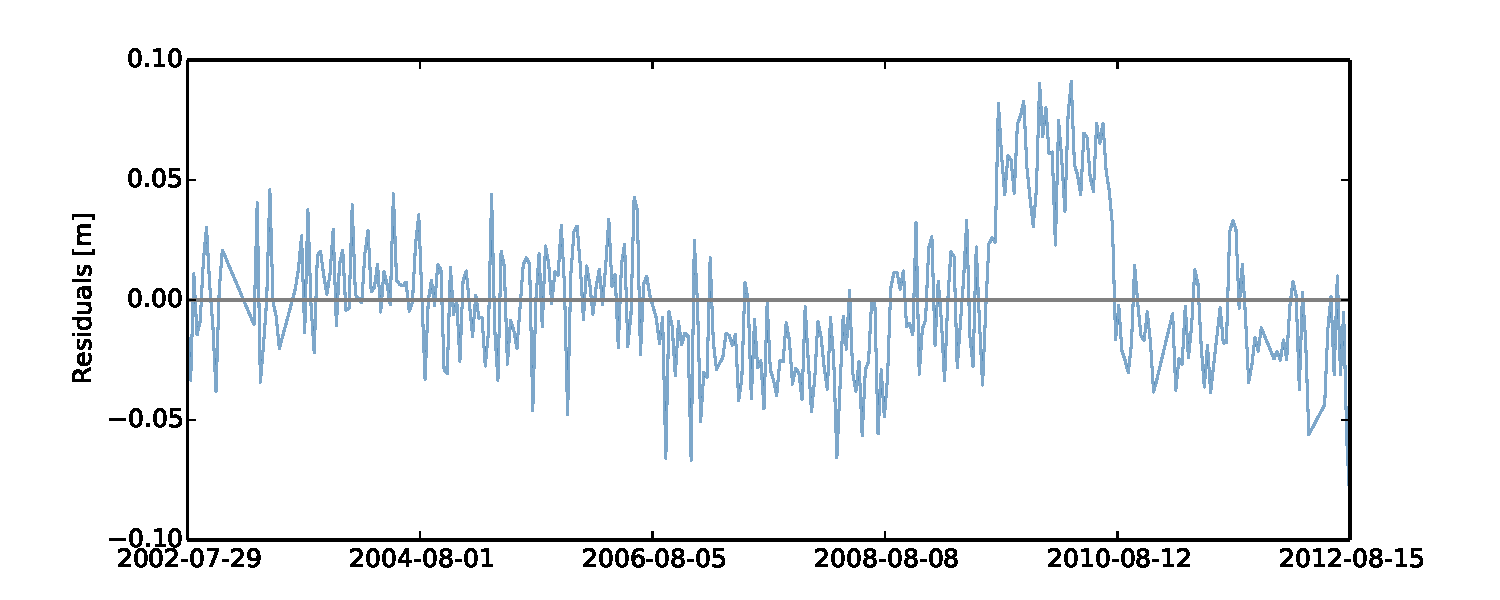
\includegraphics[width=\textwidth]{figures/splines-selected-0-residual}
	\caption{The OLS residuals are blue.}
	\label{fig:splines-selected-0-residual}
\end{figure}

Unfortunately for the south pole, the resulting fits do display some cusps and overfitting behavior. This is particularly seen at 2006 and 2008. Here the residuals haven't improved much, however interestingly enough there now appear to be a two year seasonal trend, between 2003 and 2007. 

\begin{figure}[H]
	\centering
	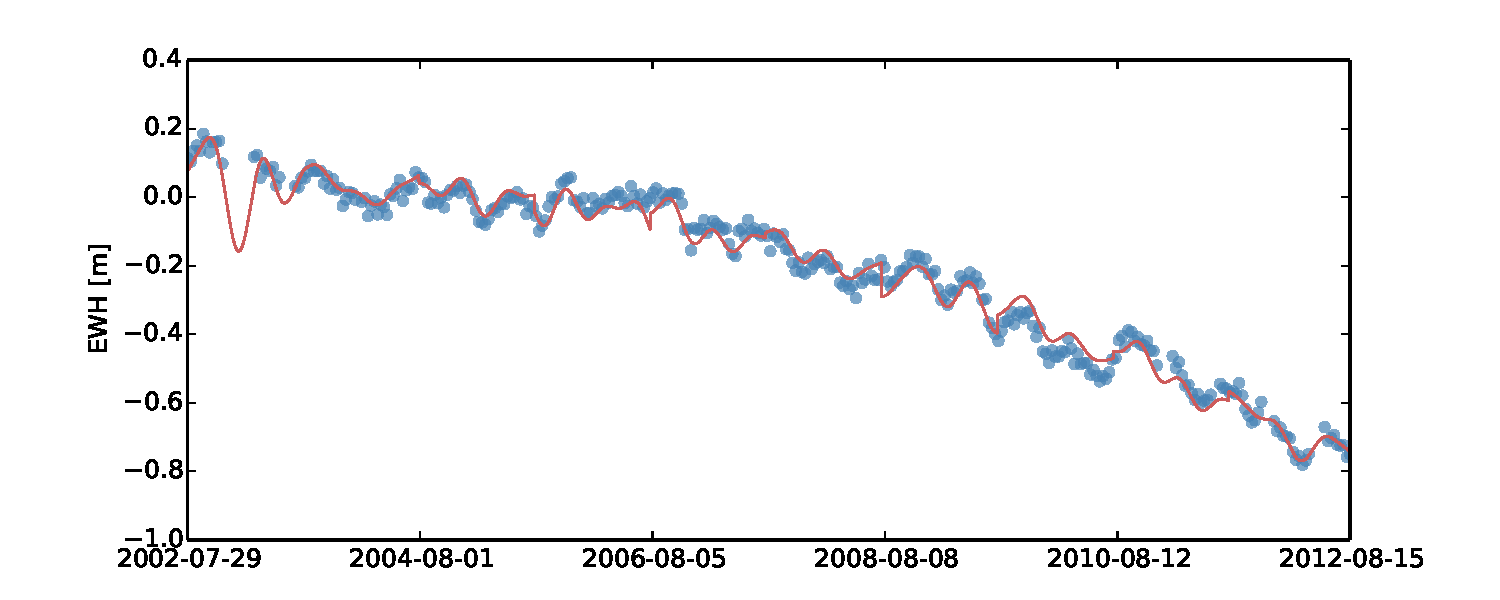
\includegraphics[width=\textwidth]{figures/splines-selected-1-fit}
	\caption{Measurements are blue, the OLS fit is red.}
	\label{fig:splines-selected-1-fit}
\end{figure}

\begin{figure}[H]
	\centering
	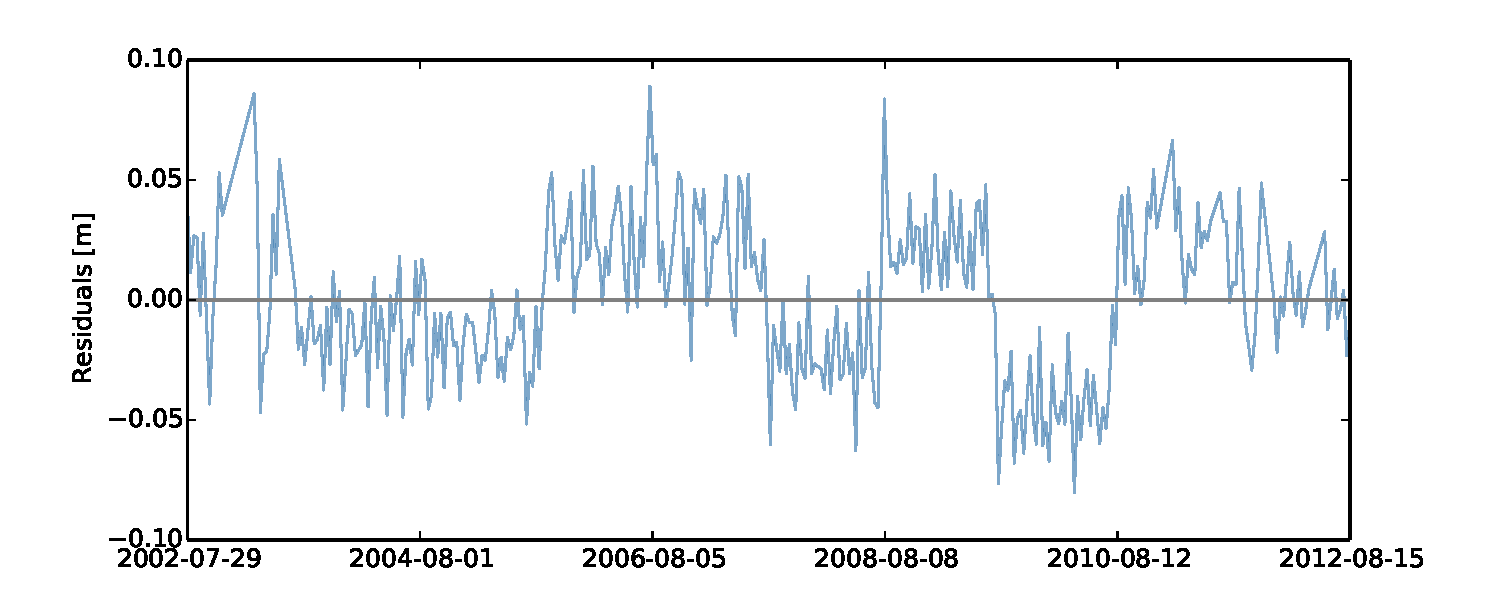
\includegraphics[width=\textwidth]{figures/splines-selected-1-residual}
	\caption{The OLS residuals are blue.}
	\label{fig:splines-selected-1-residual}
\end{figure}

\subsubsection{Ideas}
If one wanted to delve deeper into the possibilities of basis expansions and hinge function the most important thing would be to analyse where to place the knots. Even though it was here chosen to place the knots at predetermined points in time and have the knots be equal for all locations, several libraries have been developed which optimizes knot location as well polynomial degrees etc.
 A famous algorithm MARS\textregistered (multivariate adaptive regression splines) developed by Jerome Friedman, can achieve this using a 2-phase pass technique \cite{wiki-MARS} (forward, backward) but implementing the algorithm seemed out of scope for this report.
\todo[inline]{Andreas er uenlig. Den slags er brugtbart når man forventer pludselige hendelser, men ikke ved hvornår. Som fx US Air Trafic. I vores tilfælde giver det perfekt mening at modeller en svingning til et år. At introducere en ny svinging (et år) før den forige er gennemføret, gør modellen urealistisk. Istedet bør man fokusere på de curps der er nu, da det er det umidbare problem. Dette løser MARS heller ikke.}

%!TEX root=report.tex
\subsection{k-means clustering}

\subsubsection{Indentifing the amount of clusters}
Due to the size of the dataset (64800, 341), and the fact multiple simulated datasets of the same size would be needed to calculate the gap-statistic it was calculated in the HPC cluster that DTU offers for students and faculty.
It should be noted that if such a setup haven't been available, one could have used smaller subsamples of the data.
20 simulation samples of size (64800,341) was made using a multivariate uniform distribution. The following is the plot of the resulting gap statistic with its standard deviation.
\begin{figure}[H]
	\center
	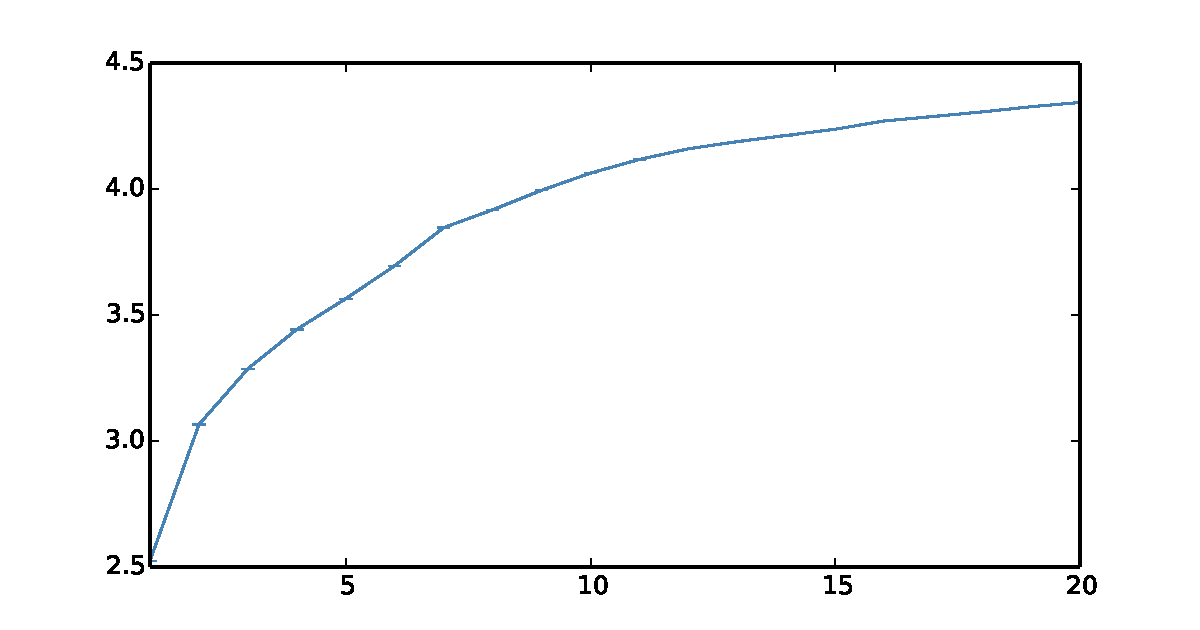
\includegraphics[width=\textwidth]{figures/kmeans-gap}
	\caption{Gap-statistics with standard deviation. Note the standard deviation is very small.}
	\label{fig:kmeans-gap}
\end{figure}

From Figure \ref{fig:kmeans-gap} its seen that according to the gap-statistics the optimal amount of cluster, is more than 20. Unfortunately such a high amount is not suitable for visualization. Instead 7 clusters have been chosen, this is based on the large slope change there can be observed in the gap-statistics graph. This is also seams like a suitable number of colors for visualization.

\begin{figure}[H]
	\center
	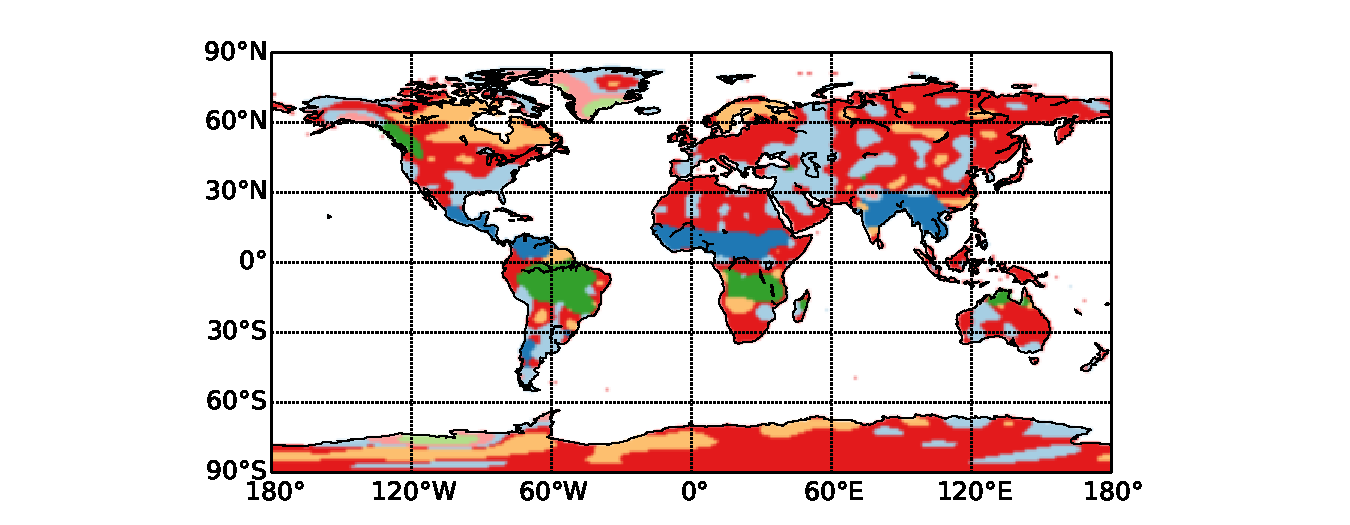
\includegraphics[width=\textwidth]{figures/kmeans-world}
	\caption{Each position is an point with belongs to the cluster, with the closest centroid.}
	\label{fig:kmeans-world}
\end{figure}
\begin{figure}[H]
	\center
	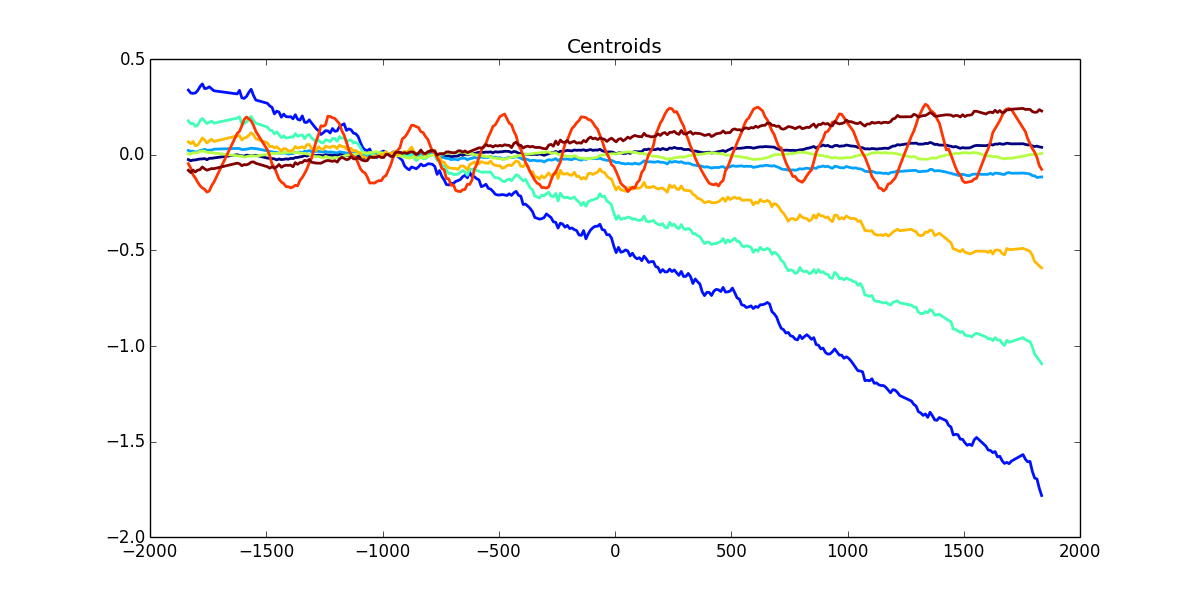
\includegraphics[width=\textwidth]{figures/kmeans-centroids}
	\caption{Cluster centroids. The colors correspond to those in Figure \ref{fig:kmeans-world}}
	\label{fig:kmeans-centroids}
\end{figure}

Comparing the two plot above a few interesting insights are gained:
\begin{itemize}
	\item Orange areas have a slight mass increase. At the south pole it appears that some of the mass loss at the edge actually moves inward towards the South Pole. This may be caused by post glacial rebound as no GIA have been performed.
	\item  Green and blue correlates with extreme and regular seasonality (i.e. rain season in Amazon Basin).
	\item Light green and pink correspond with trending mass loss. The most significant locations appear to be located around the tip of the Western Antartica along with Greenland's east coast.
\end{itemize}

%!TEX root=report.tex
\subsection{GMM clustering}
Like with K-means clustering, a matrix $X$ with dimensions ($64800 \times 341$) is used. Due to the high number of variables in GMM, the dimensionality was reduced using PCA and only selecting the first 10 PCs.
The result were not ideal, so instead a kernel version of PCA was used.

\begin{itemize}
\item The first 10 principal components was used
\item The ``Radial basis function'' was used as a kernel function
\item The amount of degree is 3
\item The gamma coefficient is set to $\sfrac{1}{341}$
\end{itemize}

\begin{figure}[H]
	\center
	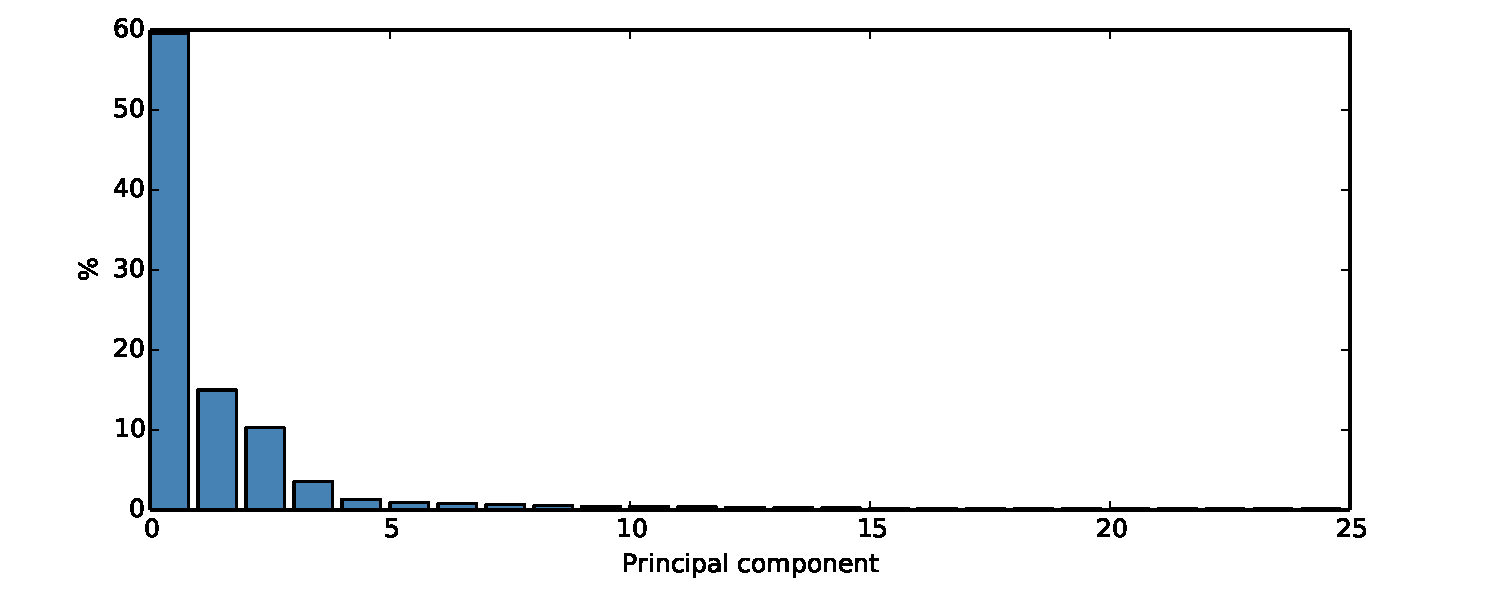
\includegraphics[width=\textwidth]{figures/gmm-pca-explaned}
	\caption{Variance explaned for the first 25 PCs, calculated as eigenvalues in $K = H(X) H(X)^T$.}
	\label{fig:gmm-pca-explaned}
\end{figure}

As seen in Figure \ref{fig:gmm-pca-explaned}, by selecting the first 10 PCs 93.18\% of the variance in the data (in the kernel space) is explained.

Next the GMM with 6 clusters was computed using the projected data. 
\begin{figure}[H]
	\center
	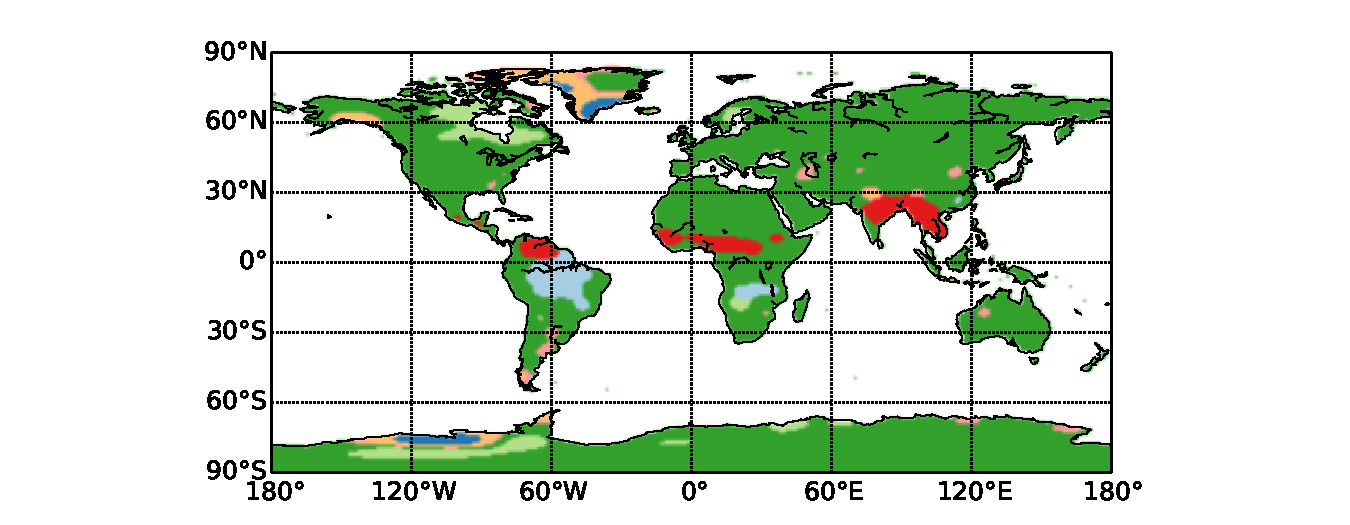
\includegraphics[width=\textwidth]{figures/gmm-world}
	\caption{Each position is a point, the color then matches a given cluster.}
\end{figure}

\begin{figure}[H]
	\center
	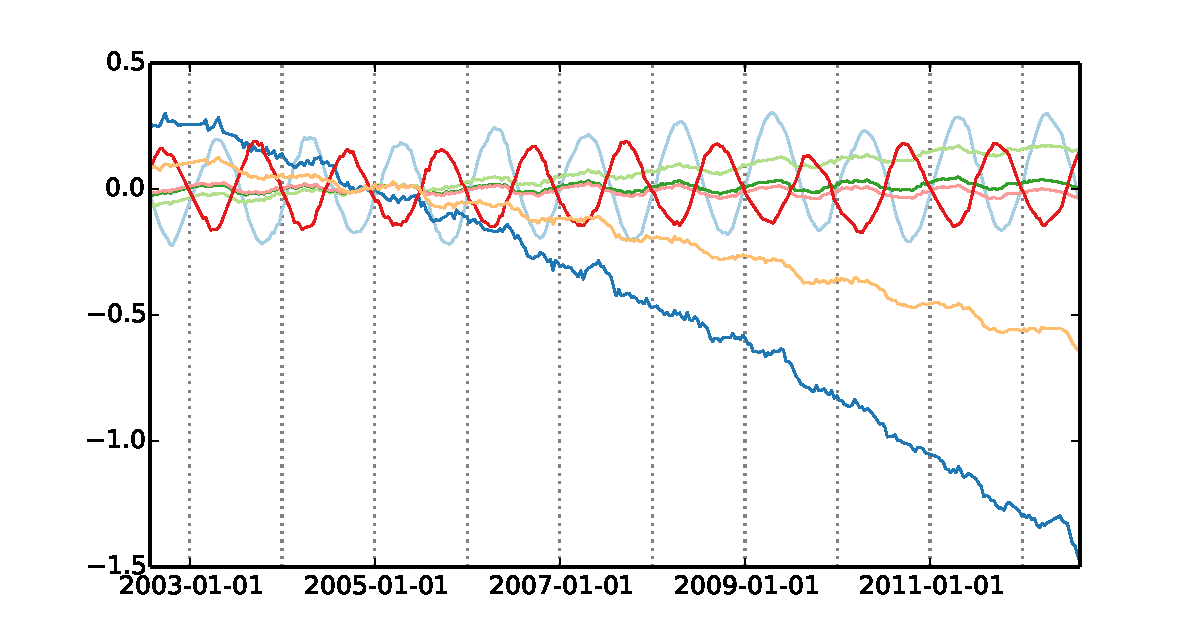
\includegraphics[width=\textwidth]{figures/gmm-centroids}
	\caption{The mean vectors for each gaussian component, projected back in the original space, using the inverse kernel PCA transformation.}
\end{figure}

Comparing the two plots above:
\begin{itemize}
	\item Light green have a slight mass increase, this was also seen in K-means clustering. Since this is observed in North America, it is likely caused by post glacial rebound.
	\item  Red and light blue correlates with extreme and regular seasonality, also very much like K-means.
	\item Blue and orange correspond with trending mass loss. With the same locations as in K-means.
	\item The big difference between GMM and K-means, is that the world graph is a lot less noisy. Only those positions with a significant different behavior than normal (green) have been caught by GMM.
	\item Finally the pink cluster is almost not noticeable and could be considered redundant. 
\end{itemize}

\pagebreak
%!TEX root=report.tex
\section{Conclusion}

The main purpose of this report was to describe mass losses or gains at the West Coast of Greenland and Western Antarctica.
Both locations were found to be losing mass.
Both location had periodic trends, but while West Greenland had soft oscillating curves Western Antarctica's mass loss was more jagged; this might suggests that ice is melting and breaking of in a more unstable pattern.
However, overall it was found that ice at the two locations was melting with approximately the same speed and with a slight difference in acceleration.

\begin{table}[H]
\centering
\begin{tabular}[H]{l | cc}
Parameter/location & Western Antarctica  & South Coast of Greenland \\ \hline
Velocity $\left[\frac{m}{day}\right]$ &  $-2.26 \cdot 10^{-4}$ & $-2.24 \cdot 10^{-4}$ \\
Acceleration $\left[\frac{m}{day^2}\right]$ &  $-1.24 \cdot 10^{-7}$ & $-8.27 \cdot 10^{-8}$ \\
\end{tabular}
\caption{Velocity and acceleration for the two analysed locations}
\end{table}

Of course these estimates depend on the selected locations and by choosing a different pair of locations, the estimates may not be exactly the same.
To get a better understanding of the patterns plots of the velocity (Figure \ref{fig:ols-world-parameter-vel}) and acceleration (Figure \ref{fig:ols-world-parameter-acc}) in a world view, was also made.
From these it is seen that Greenland and Antarctica are generally very similar in maximum magnitude of both acceleration and velocity. The most surprising observation is probably found in Greenland. Here the highest velocity is found on the east coast, but the highest acceleration is actually located on the west cost. This is not similar to Antarctica, where the highest acceleration and velocity is located at approximately the place.

Similar results were gained when using clustering algorithms to find similar locations. Here GMM with a Kernel PCA \ref{section:result-gmm} seems to give a much less noisy result than K-means \ref{section:result-kmeans}.

These results are of course influenced by the post glacial rebound. Later the ICE-5G dataset was  used to correct for this (glacial isostatic adjustment), though this NASA source \cite{NASA-GIA-incomplete} suggest that this is not enough to get useful estimates.

Attempts to improving the variance of these estimates were also made. First by using a GLS model instead of a OLS model \ref{section:result-ols-ar} and later by introducing basis expansion \ref{section:result-splines} to allow for more flexibility in the seasons. Both of these gave good results and it is even possible to combine the methods. However, in the case of the splines, even though the obtained fit was theoretically good, several cusp and movements that to the human eye looked discontinuous existed. Thus it should not be recommended to use splines with cosine and sine, without doing something to improve the continuity.

Another way to improve the variance is to reduce the amount of OLS parameters. Here the p-values and the LAR \ref{section:result-lar} model suggests that only OLS parameters down to a period of $3 \cdot \omega$ is worth keeping. At least for those selected locations.

Finally a time series model was used in form of a seasonal ARIMA \ref{section:result-ts}. The results here were disappointing in that the residuals were far from being white noise distributed. This suggests that there are exogenous inputs which affects the system in a significant way. Finding and observing those variables would possibly also allow for a better OLS estimate. 

\pagebreak
%!TEX root=report.tex
\section{Appendix}


\subsection{Tidsrækkeanalyse resultater}
\label{first-R}

Den første model baseret på graf-aflæsninger (R-output):

\begin{minipage}{1.3\textwidth}
\begin{lstlisting}
Series: xdata 
ARIMA(3,1,3)(1,1,4)[36]                    

Coefficients:
          ar1     ar2     ar3     ma1      ma2     ma3    sar1     sma1    sma2
      -0.3860  0.1239  0.0471  0.2225  -0.2783  0.0035  0.0926  -0.9147  0.1808
s.e.   0.1556     NaN     NaN  0.1673      NaN     NaN     NaN      NaN  0.0508
        sma3     sma4
      0.0980  -0.1206
s.e.  0.0466   0.0749

sigma^2 estimated as 0.0005546:  log likelihood=727.89
AIC=-1431.78   AICc=-1430.76   BIC=-1386.6

$AIC
[1] -6.435554

$AICc
[1] -6.427381

$BIC
[1] -7.315823

Warning message:
In sqrt(diag(x$var.coef)) : NaNs produced
\end{lstlisting}
\end{minipage}


\pagebreak
\printbibliography

\end{document}
